%\VignetteIndexEntry{Introduction to the rugarch package}
%\VignetteDepends{parallel}
%\VignetteKeywords{GARCH}
%\VignettePackage{rugarch}
\documentclass[11pt,a4paper]{article}
\usepackage[utf8]{inputenc}
\usepackage[round]{natbib}
\usepackage{graphicx}
\usepackage{amsmath}
\usepackage{amssymb}
\usepackage{anysize}
\usepackage{amsfonts}
\usepackage{lscape}
\usepackage{ctable}
\usepackage{subfig}
\usepackage{hyperref}
\marginsize{2cm}{2cm}{1cm}{1cm}
\setlength{\textwidth}{16cm}
\setlength{\oddsidemargin}{0cm}
\setlength{\textheight}{24cm}
\setlength{\headheight}{2cm}
\newtheorem{proof}{Proof}
\usepackage{Sweave}
\bibliographystyle{plainnat}
\begin{document}
\input{Introduction_to_the_rugarch_package-concordance}
\title{Introduction to the rugarch package.\\
(Version 1.4-3)}
\author{Alexios Ghalanos}
\date{\today}
\maketitle
\tableofcontents
\newpage
\section{Introduction}
The pioneering work of \cite{Box1994} in the area of autoregressive moving
average models paved the way for related work in the area of volatility
modelling with the introduction of ARCH and then GARCH models by \cite{Engle1982}
and \cite{Bollerslev1986}, respectively. In terms of the statistical framework,
these models provide motion dynamics for the dependency in the conditional
time variation of the distributional parameters of the mean and variance, in an
attempt to capture such phenomena as autocorrelation in returns and squared
returns. Extensions to these models have included more sophisticated dynamics
such as threshold models to capture the asymmetry in the news impact, as well
as distributions other than the normal to account for the skewness and excess
kurtosis observed in practice. In a further extension, \cite{Hansen1994}
generalized the \verb@GARCH@ models to capture time variation in the full density
parameters, with the Autoregressive Conditional Density Model\footnote{The \textbf{racd} package
is now available from my bitbucket repository.}, relaxing the assumption that the
conditional distribution of the standardized innovations is independent of the
conditioning information.

The \verb@rugarch@ package aims to provide for a comprehensive set of methods
for modelling univariate \verb@GARCH@ processes, including fitting, filtering,
forecasting, simulation as well as diagnostic tools including plots and various
tests. Additional methods such as rolling estimation, bootstrap forecasting and
simulated parameter density to evaluate model uncertainty provide a rich
environment for the modelling of these processes. This document discusses the
finer details of the included models and conditional distributions and
how they are implemented in the package with numerous examples.

The \verb@rugarch@ package is available on CRAN
(\url{http://cran.r-project.org/web/packages/rugarch/index.html}) and the
development version on bitbucket (\url{https://bitbucket.org/alexiosg}).
Some online examples and demos are available on my website
(\url{http://www.unstarched.net}).

The package is provided AS IS, without any implied warranty as to its accuracy
or suitability. A lot of time and effort has gone into the development of this
package, and it is offered under the GPL-3 license in the spirit of open
knowledge sharing and dissemination. If you do use the model in published work
DO remember to cite the package and author (type \verb@citation@("rugarch") for
the appropriate BibTeX entry) , and if you have used it and found it
useful, drop me a note and let me know.

\textbf{USE THE R-SIG-FINANCE MAILING LIST FOR QUESTIONS.}

A section on FAQ is included at the end of this document.
\section{Model Specification}
This section discusses the key step in the modelling process, namely that of the
specification. This is defined via a call to the \verb@ugarchspec@ function,
\begin{Schunk}
\begin{Sinput}
> args(ugarchspec)
\end{Sinput}
\begin{Soutput}
function (variance.model = list(model = "sGARCH", garchOrder = c(1,
    1), submodel = NULL, external.regressors = NULL, variance.targeting = FALSE),
    mean.model = list(armaOrder = c(1, 1), include.mean = TRUE,
        archm = FALSE, archpow = 1, arfima = FALSE, external.regressors = NULL,
        archex = FALSE), distribution.model = "norm", start.pars = list(),
    fixed.pars = list(), ...)
\end{Soutput}
\end{Schunk}
Thus a model, in the \verb@rugarch@ package, may be described by the dynamics of
the conditional mean and variance, and the distribution to which they belong,
which determines any additional parameters. The following sub-sections will
outline the background and details of the dynamics and distributions implemented
in the package.

\subsection{Univariate ARFIMAX Models}\label{section:umean}
The univariate GARCH specification allows to define dynamics for the conditional
mean from the general ARFIMAX model with the addition of ARCH-in-mean effects
introduced in \cite{Engle1987}.
The ARFIMAX-ARCH-in-mean specification may be formally defined as,
\begin{equation}\label{arfimax1}
\Phi(L){(1 - L)^d}({y_t} - {\mu _t}) = \Theta (L){\varepsilon _t},
\end{equation}
with the left hand side denoting the Fractional AR specification on the demeaned
data and the right hand side the MA specification on the residuals. $(L)$ is the
lag operator, $(1 - L)^d$ the long memory fractional process with $0 < d < 1$,
and equivalent to the Hurst Exponent $H$ - 0.5, and $\mu_t$ defined as,
\begin{equation}\label{arfimax2}
{\mu _t} = \mu  + \sum\limits_{i = 1}^{m - n} {{\delta _i}} {x_{i,t}} + \sum\limits_{i = m - n + 1}^m {\delta _i}{x_{i,t}}{\sigma _t} + \xi \sigma _t^k,
\end{equation}
where we allow for \verb@m@ external regressors $x$ of which $n$ (last $n$ of $m$)
may optionally be multiplied by the conditional standard deviation $\sigma_t$,
and ARCH-in-mean on either the conditional standard deviation, $k=1$ or conditional
variance $k=2$. These options can all be passed via the arguments in the \verb@mean.model@
list in the \verb@ugarchspec@ function,
\begin{itemize}
\item armaOrder 	   (default = (1,1). The order of the ARMA model.)
\item include.mean 	   (default = TRUE.  Whether the mean is modelled.)
\item archm			   (default = FALSE. The ARCH-in-mean parameter.)
\item archpow   	   (default = 1 for standard deviation, else 2 for variance.)
\item arfima	   	   (default = FALSE. Whether to use fractional differencing.)
\item external.regressors (default = NULL. A matrix of external regressors of
the same length as the data.)
\item archex           (default = FALSE. Either FALSE or integer denoting the number of external
regressors from the end of the matrix to multiply by the conditional standard deviation.).
\end{itemize}
Since the specification allows for both fixed and starting parameters to be
passed, it is useful to provide the naming convention for these here,
\begin{itemize}
\item AR parameters are 'ar1', 'ar2', ...,
\item MA parameters are 'ma1', 'ma2', ...,
\item mean parameter is 'mu'
\item archm parameter is 'archm'
\item the arfima parameter is 'arfima'
\item the external regressor parameters are 'mxreg1', 'mxreg2', ...,
\end{itemize}
Note that estimation of the mean and variance equations in the maximization of
the likelihood is carried out jointly in a single step. While it is perfectly
possible and consistent to perform a 2-step estimation, the one step approach
results in greater efficiency, particularly for smaller datasets.
\subsection{Univariate GARCH Models}\label{section:ugarch}
In GARCH models, the density function is usually written in terms of the
location and scale parameters, normalized to give zero mean and  unit variance,
\begin{equation}\label{garchdensity1}
{\alpha _t} = ({\mu_t},{\sigma_t},{\omega}),
\end{equation}
where the conditional mean is given by
\begin{equation}\label{garchdensity2}
{\mu _t} = \mu (\theta ,{x_t}) = E({y_t}|{x_t}),
\end{equation}
and the conditional variance is,
\begin{equation}\label{garchdensity3}
\sigma _t^2 = {\sigma ^2}(\theta ,{x_t}) = E({({y_t} - {\mu _t})^2}|{x_t}),
\end{equation}
with ${\omega} = \omega (\theta ,{x_t})$ denoting the remaining parameters of
the distribution, perhaps a shape and skew parameter. The conditional mean and
variance are used to scale the innovations,
\begin{equation}\label{garchdensity4}
{z_t}(\theta ) = \frac{{{y_t} - \mu (\theta ,{x_t})}}{{\sigma (\theta ,{x_t})}},
\end{equation}
having conditional density which may be written as,
\begin{equation}\label{garchdensity5}
g(z|{\omega}) = \frac{d}{{dz}}P({z_t} < z|{\omega}),
\end{equation}
and related to $f(y|\alpha)$ by,
\begin{equation}\label{garchdensity6}
f({y_t}|{\mu _t},\sigma _t^2,{\omega}) = \frac{1}{{{\sigma_t}}}g({z_t}|{\omega}).
\end{equation}

The \verb@rugarch@ package implements a rich set of univariate GARCH models and
allows for the inclusion of external regressors in the variance equation as well
as the possibility of using variance targeting as in \cite{Engle1995a}.
These options can all be passed via the arguments in the \verb@variance.model@
list in the \verb@ugarchspec@ function,
\begin{itemize}
\item model			(default = 'sGARCH' (vanilla GARCH).
Valid models are 'iGARCH', 'gjrGARCH', 'eGARCH', 'apARCH','fGARCH','csGARCH' and 'mcsGARCH').
\item garchOrder	(default = c(1,1).  The order of the GARCH model.)
\item submodel  	(default = NULL. In the case of the 'fGARCH'
omnibus model, valid choices are 'GARCH', 'TGARCH', 'GJRGARCH', 'AVGARCH',
'NGARCH', 'NAGARCH', 'APARCH' and 'ALLGARCH')
\item external.regressors (default = NULL. A matrix of external regressors of
the same length as the data).
\item variance.targeting  (default = FALSE. Whether to include variance
targeting. It is also possible to pass a numeric value instead of a logical, in which case it
is used for the calculation instead of the variance of the conditional mean equation residuals).
\end{itemize}
The rest of this section discusses the various flavors of GARCH implemented in
the package, while  Section \ref{section:distributions} discusses the
distributions implemented and their standardization for use in GARCH processes.

\subsubsection{The standard GARCH model ('sGARCH')}\label{section:sgarch}
The standard GARCH model (\cite{Bollerslev1986}) may be written as:
\begin{equation}\label{eq:sgarch}
\sigma _t^2 = \left( {\omega  + \sum\limits_{j = 1}^m {{\zeta _j}{v_{jt}}} } \right) + \sum\limits_{j = 1}^q {{\alpha _j}\varepsilon _{t - j}^2 + } \sum\limits_{j = 1}^p {{\beta _j}\sigma _{t - j}^2},
\end{equation}
with $\sigma_t^2$ denoting the conditional variance, $\omega$ the intercept
and $\varepsilon_t^2$ the residuals from the mean filtration process discussed
previously. The GARCH order is defined by $(q, p)$ (ARCH, GARCH), with possibly
\verb@m@ external regressors $v_j$ which are passed \emph{pre-lagged}.
If variance targeting is used, then $\omega$ is replaced by,
\begin{equation}\label{eq:sgarchvt}
{{\bar \sigma }^2}\left( {1 - \hat P} \right) - \sum\limits_{j = 1}^m {{\zeta _j}{{\bar v}_j}}
\end{equation}
where ${\bar \sigma}^2$ is the unconditional variance of $\varepsilon^2$ which
is consistently estimated by its sample counterpart at every iteration of the
solver following the mean equation filtration, and ${\bar v}_j$ represents the
sample mean of the $j^{th}$ external regressors in the variance equation
(assuming stationarity), and $\hat P$ is the persistence and defined below. If a
numeric value was provided to the \emph{variance.targeting} option in the specification
(instead of logical), this will be used instead of ${\bar \sigma }^2$ for the
calculation.\footnote{Note that this should represent a value related to the variance
in the plain vanilla GARCH model. In more general models such as the APARCH, this is
a value related to $\sigma^{\delta}$, which may not be obvious since $\delta$ is not
known prior to estimation, and therefore care should be taken in those cases.
Finally, if scaling is  used in the estimation (via the fit.control option), this value will
also be automatically scale adjusted by the routine.}
One of the key features of the observed behavior of financial data which GARCH
models capture is volatility clustering which may be quantified in the
persistence parameter $\hat P$. For the 'sGARCH' model this may be calculated as,
\begin{equation}\label{eq:sgarchp}
\hat P = \sum\limits_{j = 1}^q {{\alpha _j}}  + \sum\limits_{j = 1}^p {{\beta _j}}.
\end{equation}
Related to this measure is the 'half-life' (call it $h2l$) defined as the number
of days it takes for half of the expected reversion back
towards $E\left( {{\sigma ^2}} \right)$ to occur,
\begin{equation}\label{eq:sgarchh2l}
h2l = \frac{{ - {{\log }_e}2}}{{{{\log }_e}\hat P}}.
\end{equation}
Finally, the unconditional variance of the model ${\hat \sigma }^2$, and related
to its persistence, is,
\begin{equation}\label{eq:sgarchuncv}
{{\hat \sigma }^2} = \frac{{\hat \omega }}{{1 - \hat P}},
\end{equation}
where $\hat \omega$ is the estimated value of the intercept from the GARCH model.
The naming conventions for passing fixed or starting parameters for this model
are:
\begin{itemize}
\item ARCH(q) parameters are 'alpha1', 'alpha2', ...,
\item GARCH(p) parameters are 'beta1', 'beta2', ...,
\item variance intercept parameter is 'omega'
\item the external regressor parameters are 'vxreg1', 'vxreg2', ...,
\end{itemize}

\subsubsection{The integrated GARCH model ('iGARCH')}\label{section:igarch}
The integrated GARCH model (see \cite{Engle1986}) assumes that the
persistence $\hat P = 1$, and imposes this during the estimation procedure.
Because of unit persistence, none of the other results can be calculated
(i.e. unconditional variance, half life etc). The stationarity of the model has
been established in the literature, but one should investigate the possibility
of omitted structural breaks before adopting the iGARCH as the model of choice.
The way the package enforces the sum of the ARCH and GARCH parameters to be 1,
is by subtracting $1 - \sum\limits_{i = 1}^q {{\alpha _i} - } \sum\limits_{i > 1}^p {{\beta _i}}$,
so that the last beta is never estimated but instead calculated.
\subsubsection{The exponential GARCH model}\label{section:egarch}
The exponential model of \cite{Nelson1991} is defined as,
\begin{equation}\label{eq:egarch}
{\log _e}\left( {\sigma _t^2} \right) = \left( {\omega  + \sum\limits_{j = 1}^m {{\zeta _j}{v_{jt}}} } \right) + \sum\limits_{j = 1}^q {\left( {{\alpha _j}{z_{t - j}} + {\gamma _j}\left( {\left| {{z_{t - j}}} \right| - E\left| {{z_{t - j}}} \right|} \right)} \right) + } \sum\limits_{j = 1}^p {{\beta _j}{{\log }_e}\left( {\sigma _{t - j}^2} \right)}
\end{equation}
where the coefficient $\alpha_j$ captures the sign effect and $\gamma_j$ the
size effect. The expected value of the absolute standardized innovation, $z_t$
is,
\begin{equation}\label{eq:egarchE}
E\left| {{z_t}} \right| = \int\limits_{ - \infty }^\infty  {\left| z \right|} f\left( {z,0,1,...} \right)dz
\end{equation}
The persistence $\hat P$ is given by,
\begin{equation}\label{eq:egarchp}
\hat P = \sum\limits_{j = 1}^p {{\beta _j}}.
\end{equation}
If variance targeting is used, then $\omega$ is replaced by,
\begin{equation}\label{eq:egarchvt}
{\log _e}\left( {{{\bar \sigma }^2}} \right)\left( {1 - \hat P} \right) - \sum\limits_{j = 1}^m {{\zeta _j}{{\bar v}_j}}
\end{equation}
The unconditional variance and half life follow from the persistence parameter
and are calculated as in Section \ref{section:sgarch}.

\subsubsection{The GJR-GARCH model ('gjrGARCH')}\label{section:gjrgarch}
The GJR GARCH model of \cite{Glosten1993} models positive and negative shocks on
the conditional variance asymmetrically via the use of the indicator function $I$,
\begin{equation}\label{eq:gjrgarch}
\sigma _t^2 = \left( {\omega  + \sum\limits_{j = 1}^m {{\zeta _j}{v_{jt}}} } \right) + \sum\limits_{j = 1}^q {\left( {{\alpha _j}\varepsilon _{t - j}^2 + {\gamma _j}{{I}_{t - j}}\varepsilon _{t - j}^2} \right) + } \sum\limits_{j = 1}^p {{\beta _j}\sigma _{t - j}^2},
\end{equation}
where $\gamma_j$ now represents the 'leverage' term. The indicator function $I$
takes on value of 1 for $\varepsilon \le 0$ and 0 otherwise. Because of the
presence of the indicator function, the persistence of the model now crucially
depends on the asymmetry of the conditional distribution used. The persistence
of the model $\hat P$ is,
\begin{equation}\label{eq:gjrgarchp}
\hat P = \sum\limits_{j = 1}^q {{\alpha _j}}  + \sum\limits_{j = 1}^p {{\beta _j} + } \sum\limits_{j = 1}^q {{\gamma _j}\kappa },
\end{equation}
where $\kappa$ is the expected value of the standardized residuals $z_t$ below
zero (effectively the probability of being below zero),
\begin{equation}\label{eq:gjrgarchkappa}
\kappa  = E\left[ {{I_{t - j}}z_{t - j}^2} \right] = \int\limits_{ - \infty }^0 {f\left( {z,0,1,...} \right)dz}
\end{equation}
where $f$ is the standardized conditional density with any additional skew and
shape parameters $(\dots)$. In the case of symmetric distributions the value of
$\kappa$ is simply equal to $0.5$. The variance targeting, half-life and
unconditional variance follow from the persistence parameter and are calculated
as in Section \ref{section:sgarch}.
The naming conventions for passing fixed or starting parameters for this model
are:
\begin{itemize}
\item ARCH(q) parameters are 'alpha1', 'alpha2', ...,
\item Leverage(q) parameters are 'gamma1', 'gamma2', ...,
\item GARCH(p) parameters are 'beta1', 'beta2', ...,
\item variance intercept parameter is 'omega'
\item the external regressor parameters are 'vxreg1', 'vxreg2', ...,
\end{itemize}
Note that the Leverage parameter follows the order of the ARCH parameter.

\subsubsection{The asymmetric power ARCH model ('apARCH')}\label{section:aparch}
The asymmetric power ARCH model of \cite{Ding1993} allows for both leverage and
the Taylor effect, named after \cite{Taylor1986} who observed that the sample
autocorrelation of absolute returns was usually larger than that of squared
returns.
\begin{equation}\label{eq:aparch}
\sigma _t^\delta  = \left( {\omega  + \sum\limits_{j = 1}^m {{\zeta _j}{v_{jt}}} } \right) + \sum\limits_{j = 1}^q {{\alpha _j}{{\left( {\left| {{\varepsilon _{t - j}}} \right| - {\gamma _j}{\varepsilon _{t - j}}} \right)}^\delta } + } \sum\limits_{j = 1}^p {{\beta _j}\sigma _{t - j}^\delta }
\end{equation}
where $\delta  \in {\mathbb{R}^ + }$, being a Box-Cox transformation of $\sigma_t$,
and $\gamma_j$ the coefficient in the leverage term. Various submodels arise
from this model:
\begin{itemize}
\item The simple GARCH model of \cite{Bollerslev1986} when $\delta=2$ and $\gamma_j=0$.
\item The Absolute Value GARCH (AVGARCH) model of \cite{Taylor1986} and \cite{Schwert1990} when $\delta=1$ and $\gamma_j=0$.
\item The GJR GARCH (GJRGARCH) model of \cite{Glosten1993} when $\delta=2$.
\item The Threshold GARCH (TGARCH) model of \cite{Zakoian1994} when $\delta=1$.
\item The Nonlinear ARCH model of \cite{Higgins1992} when $\gamma_j=0$ and $\beta_j=0$.
\item The Log ARCH model of \cite{Geweke1986} and \cite{Pantula1986} when $\delta  \to 0$.
\end{itemize}
The persistence of the model is given by,
\begin{equation}\label{eq:aparchp}
\hat P = \sum\limits_{j = 1}^p {{\beta_j} + } \sum\limits_{j = 1}^q {{\alpha_j}} {\kappa_j}
\end{equation}
where $\kappa_j$ is the expected value of the standardized residuals $z_t$ under
the Box-Cox transformation of the term which includes the leverage coefficient
$\gamma_j$,
\begin{equation}\label{eq:aparchkappa}
\kappa_j  = E{\left( {\left| z \right| - {\gamma _j}z} \right)^\delta } = \int\limits_{ - \infty }^\infty  {{{\left( {\left| z \right| - {\gamma _j}z} \right)}^\delta }f\left( {z,0,1,...} \right)dz}
\end{equation}
If variance targeting is used, then $\omega$ is replaced by,
\begin{equation}\label{eq:aparchvt}
{{\bar \sigma }^\delta }\left( {1 - \hat P} \right) - \sum\limits_{j = 1}^m {{\zeta _j}{{\bar v}_j}}.
\end{equation}
Finally, the unconditional variance of the model ${\hat \sigma }^2$ is,
\begin{equation}\label{eq:aparchuncv}
{{\hat \sigma }^2} = {\left( {\frac{{\hat \omega }}{{1 - \hat P}}} \right)^{2/\delta }}
\end{equation}
where $\hat \omega$ is the estimated value of the intercept from the GARCH model.
The half-life follows from the persistence parameter and is calculated as in
Section \ref{section:sgarch}. The naming conventions for passing fixed or
starting parameters for this model are:
\begin{itemize}
\item ARCH(q) parameters are 'alpha1', 'alpha2', ...,
\item Leverage(q) parameters are 'gamma1', 'gamma2', ...,
\item Power parameter is 'delta',
\item GARCH(p) parameters are 'beta1', 'beta2', ...,
\item variance intercept parameter is 'omega'
\item the external regressor parameters are 'vxreg1', 'vxreg2', ...,
\end{itemize}
In particular, to obtain any of the submodels simply pass the appropriate
parameters as fixed.

\subsubsection{The family GARCH model ('fGARCH')}\label{section:fgarch}
The family GARCH model of \cite{Hentschel1995} is another omnibus model which
subsumes some of the most popular GARCH models. It is similar to the apARCH
model, but more general since it allows the decomposition of the residuals in
the conditional variance equation to be driven by different powers for $z_t$
and $\sigma_t$ and also allowing for both shifts and rotations in the news
impact curve, where the shift is the main source of asymmetry for small shocks
while rotation drives large shocks.
\begin{equation}\label{eq:fgarch}
\sigma _t^\lambda  = \left( {\omega  + \sum\limits_{j = 1}^m {{\zeta _j}{v_{jt}}} } \right) + \sum\limits_{j = 1}^q {{\alpha _j}\sigma _{t - j}^\lambda {{\left( {\left| {{z_{t - j}} - {\eta _{2j}}} \right| - {\eta _{1j}}\left( {{z_{t - j}} - {\eta _{2j}}} \right)} \right)}^\delta } + } \sum\limits_{j = 1}^p {{\beta _j}\sigma _{t - j}^\lambda }
\end{equation}
which is a Box-Cox transformation for the conditional standard deviation whose
shape is determined by $\lambda$, and the parameter $\delta$ transforms the
absolute value function which it subject to rotations and shifts through the
$\eta_{1j}$ and $\eta_{2j}$ parameters respectively. Various submodels arise
from this model, and are passed to the \verb@ugarchspec@ 'variance.model' list
via the submodel option,
\begin{itemize}
\item The simple GARCH model of \cite{Bollerslev1986} when $\lambda=\delta=2$ and $\eta_1j=\eta_2j=0$ (submodel = 'GARCH').
\item The Absolute Value GARCH (AVGARCH) model of \cite{Taylor1986} and \cite{Schwert1990} when $\lambda=\delta=1$ and $|{{\eta _{1j}}}| \leq 1$ (submodel = 'AVGARCH').
\item The GJR GARCH (GJRGARCH) model of \cite{Glosten1993} when $\lambda=\delta=2$ and $\eta_{2j}=0$ (submodel = 'GJRGARCH').
\item The Threshold GARCH (TGARCH) model of \cite{Zakoian1994} when $\lambda=\delta=1$, $\eta_{2j}=0$ and $|{{\eta _{1j}}}| \leq 1$ (submodel = 'TGARCH').
\item The Nonlinear ARCH model of \cite{Higgins1992} when $\delta=\lambda$ and  $\eta_1j=\eta_2j=0$ (submodel = 'NGARCH').
\item The Nonlinear Asymmetric GARCH model of \cite{Engle1993} when $\delta=\lambda=2$ and $\eta_1j=0$ (submodel = 'NAGARCH').
\item The Asymmetric Power ARCH model of \cite{Ding1993} when $\delta=\lambda$, $\eta_{2j}=0$ and $|{{\eta _{1j}}}| \leq 1$ (submodel = 'APARCH').
\item The Exponential GARCH model of \cite{Nelson1991} when $\delta=1$, $\lambda=0$ and $\eta_{2j}=0$ (not implemented as a submodel of fGARCH).
\item The Full fGARCH model of \cite{Hentschel1995} when $\delta=\lambda$ (submodel = 'ALLGARCH').
\end{itemize}
The persistence of the model is given by,
\begin{equation}\label{eq:fgarchp}
\hat P = \sum\limits_{j = 1}^p {{\beta_j} + } \sum\limits_{j = 1}^q {{\alpha_j}} {\kappa_j}
\end{equation}
where $\kappa_j$ is the expected value of the standardized residuals $z_t$ under
the Box-Cox transformation of the absolute value asymmetry term,
\begin{equation}\label{eq:fgarchkappa}
{\kappa _j} = E{\left( {\left| {{z_{t - j}} - {\eta _{2j}}} \right| - {\eta _{1j}}\left( {{z_{t - j}} - {\eta _{2j}}} \right)} \right)^\delta } = \int\limits_{ - \infty }^\infty  {{{\left( {\left| {z - {\eta _{2j}}} \right| - {\eta _{1j}}\left( {z - {\eta _{2j}}} \right)} \right)}^\delta }f\left( {z,0,1,...} \right)dz}
\end{equation}

If variance targeting is used, then $\omega$ is replaced by,
\begin{equation}\label{eq:fgarchvt}
{{\bar \sigma }^\lambda }\left( {1 - \hat P} \right) - \sum\limits_{j = 1}^m {{\zeta _j}{{\bar v}_j}}
\end{equation}
Finally, the unconditional variance of the model ${\hat \sigma }^2$ is,
\begin{equation}\label{eq:fgarchuncv}
{{\hat \sigma }^2} = {\left( {\frac{{\hat \omega }}{{1 - \hat P}}} \right)^{2/\lambda }}
\end{equation}
where $\hat \omega$ is the estimated value of the intercept from the GARCH model.
The half-life follows from the persistence parameter and is calculated as in
Section \ref{section:sgarch}.
The naming conventions for passing fixed or starting parameters for this model
are:
\begin{itemize}
\item ARCH(q) parameters are 'alpha1', 'alpha2', ...,
\item Asymmetry1(q) - rotation - parameters are 'eta11', 'eta12', ...,
\item Asymmetry2(q) - shift - parameters are 'eta21', 'eta22', ...,
\item Asymmetry Power parameter is 'delta',
\item Conditional Sigma Power parameter is 'lambda',
\item GARCH(p) parameters are 'beta1', 'beta2', ...,
\item variance intercept parameter is 'omega'
\item the external regressor parameters are 'vxreg1', 'vxreg2', ...,
\end{itemize}


\subsubsection{The Component sGARCH model ('csGARCH')}\label{section:csgarch}
The model of \cite{Lee1999} decomposes the conditional variance into a
permanent and transitory component so as to investigate the long- and short-run
movements of volatility affecting securities. Letting $q_t$ represent the permanent
component of the conditional variance, the component model can then be written
as:
\begin{equation}
\begin{gathered}
  \sigma _t^2 = {q_t} + \sum\limits_{j = 1}^q {{\alpha _j}\left( {\varepsilon _{t - j}^2 - {q_{t - j}}} \right) + } \sum\limits_{j = 1}^p {{\beta _j}\left( {\sigma _{t - j}^2 - {q_{t - j}}} \right)}  \hfill \\
  {q_t} = \omega  + \rho {q_{t - 1}} + \phi \left( {\varepsilon _{t - 1}^2 - \sigma _{t - 1}^2} \right) \hfill \\
\end{gathered}
\end{equation}
where effectively the intercept of the GARCH model is now time-varying
following first order autoregressive type dynamics. The difference between
the conditional variance and its trend, $\sigma_{t - j}^2 - q_{t-j}$ is the
transitory component of the conditional variance. The conditions for the
non-negativity of the conditional variance are given in \cite{Lee1999} and
imposed during estimation by the stationarity option in the fit.control list
of the \verb@ugarchfit@ method, and related to the stationarity conditions
that the sum of the ($\alpha$,$\beta$) coefficients be less than 1 and that $\rho<1$
(effectively the persistence of the transitory and permanent components).\\
The multistep, $n>1$ ahead forecast of the conditional variance proceeds as follows:
\begin{equation}
\begin{gathered}
  {E_{t - 1}}\left( {\sigma _{t + n}^2} \right) = {E_{t - 1}}\left( {{q_{t + n}}} \right) + \sum\limits_{j = 1}^q {{\alpha _j}\left( {\varepsilon _{t + n - j}^2 - {q_{t + n - j}}} \right) + } \sum\limits_{j = 1}^p {{\beta _j}\left( {\sigma _{t + n - j}^2 - {q_{t + n - j}}} \right)}  \hfill \\
  {E_{t - 1}}\left( {\sigma _{t + n}^2} \right) = {E_{t - 1}}\left( {{q_{t + n}}} \right) + \sum\limits_{j = 1}^q {{\alpha _j}{E_{t - 1}}\left[ {\varepsilon _{t + n - j}^2 - {q_{t + n - j}}} \right] + } \sum\limits_{j = 1}^p {{\beta _j}{E_{t - 1}}\left[ {\sigma _{t + n - j}^2 - {q_{t + n - j}}} \right]}  \hfill \\
\end{gathered}
\end{equation}
However, ${E_{t - 1}}\left[ {\varepsilon _{t + n - j}^2} \right] = {E_{t - 1}}\left[ {\sigma _{t + n - j}^2} \right]$, therefore:
\begin{equation}
\begin{gathered}
  {E_{t - 1}}\left( {\sigma _{t + n}^2} \right) = {E_{t - 1}}\left( {{q_{t + n}}} \right) + \sum\limits_{j = 1}^q {{\alpha _j}{E_{t - 1}}\left[ {\sigma _{t + n - j}^2 - {q_{t + n - j}}} \right] + } \sum\limits_{j = 1}^p {{\beta _j}{E_{t - 1}}\left[ {\sigma _{t + n - j}^2 - {q_{t + n - j}}} \right]}  \hfill \\
  {E_{t - 1}}\left( {\sigma _{t + n}^2} \right) = {E_{t - 1}}\left( {{q_{t + n}}} \right) + {\left[ {\sum\limits_{j = 1}^{\max (p,q)} {\left( {{\alpha _j} + {\beta _j}} \right)} } \right]^n}\left( {\sigma _t^2 - {q_t}} \right) \hfill \\
\end{gathered}
\end{equation}
The permanent component forecast can be represented as:
\begin{align}
  {E_{t - 1}}\left[ {{q_{t + n}}} \right] & = \omega  + \rho {E_{t - 1}}\left[ {{q_{t + n - 1}}} \right] + \phi {E_{t - 1}}\left[ {\varepsilon _{t + n - j}^2 - \sigma _{t + n - j}^2} \right] \hfill \\
   & = \omega  + \rho {E_{t - 1}}\left[ {{q_{t + n - 1}}} \right]\hfill \\
   & = \omega  + \rho \left[ {\omega  + \rho {E_{t - 1}}\left[ {{q_{t + n - 2}}} \right]} \right] \hfill \\
   & = \dots \hfill \\
   & = \left( {1 + p + \dots + {\rho ^{n - 1}}} \right)\omega  + {\rho ^n}{q_t} \hfill \\
   & = \frac{{1 - {\rho ^n}}}{{1 - \rho }}\omega  + {\rho ^n}{q_t} \hfill \\
\end{align}
As $n \to \infty$ the unconditional variance is:
\begin{equation}
{E_{t - 1}}\left[ {\sigma _{t + n}^2} \right] = {E_{t - 1}}\left[ {{q_{t + n}}} \right] = \frac{\omega }{{1 - \rho }}
\end{equation}
In the \verb@rugarch@ package, the parameters $\rho$ and $\phi$ are
represented by $\eta_{11}$('eta11') and $\eta_{21}$('eta21') respectively.
\subsubsection{The Multiplicative Component sGARCH model ('mcsGARCH')}\label{section:mcsgarch}
A key problem with using GARCH models for intraday data is the seasonality in the absolute returns observed at the beginning and end of the trading session. For regularly sampled time intervals (1-min, 5-min etc.), a number of models have tried to either 'de-seasonalize' the residuals and then fit the GARCH model by using for instance a Flexible Fourier method as in \cite{Andersen1997} or incorporate seasonality directly into the model as in the Periodic GARCH model of \cite{Bollerslev1996}. A rather simple and parsimonious approach to the de-seasonalization was recently presented in \cite{Engle2012} (henceforth ES2012). Consider the continuously compounded return $r_{t,i}$, where $t$ denotes the day and $i$ the regularly spaced time interval at which the return was calculated. Under this model, the conditional variance is a multiplicative product of daily, diurnal and stochastic (intraday) components, so that the return process may be represented as:
\begin{equation}\label{mcs1}
\begin{gathered}
  {r_{t,i}} = {\mu _{t,i}} + {\varepsilon _{t,i}} \hfill \\
  {\varepsilon _{t,i}} = \left( {{q_{t,i}}{\sigma _t}{s_i}} \right){z_{t,i}} \hfill \\
\end{gathered}
\end{equation}
where $q_{t,i}$ is the stochastic intraday volatility, $\sigma_t$ a daily exogenously determined forecast volatility, $s_i$ the diurnal volatility in each regularly spaced interval $i$, $z_{t,i}$ the i.i.d (0,1) standardized innovation which conditional follows some appropriately chosen distribution. In ES2012, the forecast volatility $\sigma_t$ is derived from a multifactor risk model externally, but it is just as possible to generate such forecasts from a daily GARCH model. The seasonal (diurnal) part of the process is defined as:
\begin{equation}\label{mcs2}
{s_i} = \frac{1}{T}\sum\limits_{t = 1}^T {\left( {\varepsilon _{_{t,i}}^2/\sigma _t^2} \right)}.
\end{equation}
Dividing the residuals by the diurnal and daily volatility gives the normalized residuals ($\bar \varepsilon$):
\begin{equation}\label{mcs3}
{{\bar \varepsilon }_{t,i}} = {\varepsilon _{t,i}}/\left( {{\sigma _t}{s_i}} \right)
\end{equation}
which may then be used to generate the stochastic component of volatility $q_{t,i}$ which assuming a simple vanilla GARCH model has the following motion dynamics:
\begin{equation}\label{mcs4}
q_{t,i}^2 = \left( {\omega  + \sum\limits_{j = 1}^m {{\zeta _j}{v_{jt}}} } \right) + \sum\limits_{j = 1}^p {{\alpha _j}\bar \varepsilon _{t - j}^2 + } \sum\limits_{j = 1}^q {{\beta _j}q_{t - j}^2}
\end{equation}
see Section \ref{section:sgarch} for details.
In the \verb@rugarch@ package, unlike the paper of ES2012, the conditional mean and variance equations (and hence the diurnal component on the residuals from the conditional mean filtration) are estimated jointly. Furthermore, and unlike ES2012, it is possible to include ARMAX dynamics in the conditional mean, though because of the complexity of the model and its use of time indices, ARCH-m is not currently allowed, but may be included once the xts package is fully translated to Rcpp. Finally, as an additional point of departure from ES2012, the diurnal component calculation uses the median instead of the mean which was found to provide for a more robust alternative, particularly given the type and size of datasets typically used [changed in version 1.2-3].
As currently stands, the model has methods for estimation (ugarchfit), filtering (ugarchfilter), forecast from fit (ugarchforecast) but not from spec (secondary dispatch method), simulation from fit (ugarchsim) but not from spec (ugarchpath), rolling estimation (ugarchroll) but not the bootstrap (ugarchboot). Some of the plots, which depend on the xts package will not render nicely since plot.xts does not play well with intraday data. Some plots however such as VaRplot have been amended to properly display intraday data coming from an xts object, and more may be added as time allows. An extensive example of the model may be found on \url{http://www.unstarched.net}.
The paper by ES2012 is currently freely available here: \url{http://jfec.oxfordjournals.org/content/10/1/54.full}.

\subsubsection{The realized GARCH model ('realGARCH')}\label{section:realgarch}
While the previous section discussed the modelling of intraday returns using a multiplicative component GARCH model, this section deals with the inclusion of realized measures of volatility
in a GARCH modelling setup. The realized GARCH (realGARCH) model of \cite{Hansen2012} (henceforth HHS2012) provides for an excellent framework for the joint modelling of returns and realized measures of volatility. Unlike the naive augmentation of GARCH processes by a realized measures, the realGARCH model relates the observed realized measure to the latent volatility via a measurement equation, which also includes asymmetric reaction to shocks, making for a very flexible and rich representation. Formally, let:
\begin{equation}
\begin{gathered}
  {y_t} = {\mu _t} + {\sigma _t}{z_t},{\text{  }}{z_t} \sim i.i.d\left( {0,1} \right) \hfill \\
  \log \sigma _t^2 = \omega  + \sum\limits_{i = 1}^q {{\alpha _i}\log {r_{t - i}} + \sum\limits_{i = 1}^p {{\beta _i}\log \sigma _{t - i}^2} }  \hfill \\
  \log r_t = \xi  + \delta \log \sigma _t^2 + \tau \left( {{z_t}} \right) + {u_t},{\text{  }}{u_t} \sim N\left( {0,\lambda } \right) \hfill \\
\end{gathered}
\end{equation}
where we have defined the dynamics for the returns ($y_t$), the log of the conditional variance ($\sigma^2_t$) and the log of the realized measure ($r_t$).\footnote{In the original paper by HHS2012, the notation is slightly different as I have chosen to re-use some of the symbols/variables already in the rugarch specification. For completeness, the differences are noted:
\begin{itemize}
\item $y_t$ (rugarch)  = $r_t$ (HHS2012)
\item $\alpha$ (rugarch)  = $\gamma$ (HHS2012)
\item $\sigma^2_t$ (rugarch) = $h_t$ (HHS2012)
\item $r_t$ (rugarch)  = $x_t$ (HHS2012)
\item $\delta$ (rugarch)   = $\varphi$ (HHS2012)
\item $\eta_1$ (rugarch) = $\tau_1$ (HHS2012)
\item $\eta_2$ (rugarch) = $\tau_2$ (HHS2012)
\item $\lambda$ (rugarch)  = $\sigma_u$ (HHS2012)
\end{itemize}
}
The asymmetric reaction to shocks comes via the $\tau\left(.\right)$ function which is based on the Hermite polynomials and truncated at the second level to give a simple quadratic form:
\begin{equation}
\tau\left(z_t\right) = \eta_1z_t + \eta_2\left(z^2_t-1\right)
\end{equation}
which has the very convenient property that $E\tau\left(z_t\right)=0$. The function also forms the basis for the creation of a type of news impact curve $\nu \left( z \right)$, defined as:
\begin{equation}
\begin{gathered}
  \nu \left( z \right) = E\left[ {\log {\sigma _t}\left| {{z_{t - 1}} = z} \right.} \right] - E\left[ {\log {\sigma _t}} \right] = \delta \tau \left( z \right) \hfill \\
\end{gathered}
\end{equation}
so that $100\times\nu\left(z\right)$ is the percent change in volatility as a function of the standardized innovations.

A key feature of this model is that it preserves the ARMA structure which characterize many standard GARCH models and adapted here from Proposition 1 of the HHS2012 paper:
\begin{equation}
\begin{gathered}
  \log \sigma _t^2 = {\mu _\sigma } + \sum\limits_{i = 1}^{p \vee q} {\left( {\delta {\alpha _i} + {\beta _i}} \right)\log \sigma _{t - 1}^2 + } \sum\limits_{j = 1}^q {{\alpha _j}{w_{t - j}}}  \hfill \\
  \log {r_t} = {\mu _r} + \sum\limits_{i = 1}^{p \vee q} {\left( {\delta {\alpha _i} + {\beta _i}} \right)\log {r_{t - 1}} + {w_t}}  - \sum\limits_{j = 1}^{p \vee q} {{\beta _j}{w_{t - j}}}  \hfill \\
  {\mu _\sigma } = \omega  + \xi \sum\limits_{i = 1}^q {{\alpha _i}} ,{\mu _r} = \delta \omega  + \left( {1 - \sum\limits_{i = 1}^p {{\beta _i}} } \right)\xi  \hfill \\
\end{gathered}
\end{equation}
where $w_t=\tau\left(z_t\right)+u_t$, ${\mu _\sigma } = \omega  + \xi \sum\limits_{i = 1}^q {{\alpha _i}}$ and ${\mu _r} = \delta \omega  + \left( {1 - \sum\limits_{i = 1}^p {{\beta _i}} } \right)\xi$, and the convention ${\beta _i} = {\alpha _j} = 0$ for $i>p$ and $j<p$. It is therefore a simple matter to show that the persistence ($\hat P$) of the process is given by:
\begin{equation}
\hat P = \sum\limits_{i = 1}^p {{\beta _i} + } \delta \sum\limits_{i = 1}^q {{\alpha _i}}
\end{equation}
while the unconditional (long-run) variance may be written as:
\begin{equation}
{\hat \sigma ^2} = \frac{{\omega  + \xi \sum\limits_{i = 1}^q {{\alpha _i}} }}
{{1 - \hat P}}
\end{equation}
The joint likelihood of the model, made up of the returns and measurement equation, is given by:
\begin{equation}
  \log L\left( {\left\{ {{y_t},{r_t}} \right\}_{t = 1}^T;\theta } \right) = \sum\limits_{t = 1}^T {\log f\left( {{y_t},{r_t}\left| {\mathcal{F}_{t - 1}} \right.} \right)}  \hfill \\
\end{equation}
While not standard for MLE, the independence of $z_t$ and $u_t$ means that we can factorize the joint density into:
\begin{equation}
\log f\left( {{y_t},{r_t}\left| {\mathcal{F}_{t - 1}} \right.} \right) = \underbrace {\log \left( {{y_t}\left| {\mathcal{F}_{t - 1}} \right.} \right)}_{\log l\left( y \right)} + \underbrace {\left( {{r_t}\left| {{y_t},\mathcal{F}_{t - 1}} \right.} \right)}_{\log l\left( {r\left| y \right.} \right)} \hfill \\
\end{equation}
which makes comparison with other GARCH models possible (using $\log l\left(y\right)$).
Finally, multiperiod forecasts have a nice VARMA type representation ${Y_t} = A{Y_{t - 1}} + b + {\varepsilon _t}$, where:
\begin{equation}
\begin{gathered}
  {Y_t} = \left[ {\begin{array}{*{20}{c}}
   {\log \sigma _t^2}  \\
   .  \\
   .  \\
   .  \\
   {\log \sigma _{t - p + 1}^2}  \\
   {\log {r_t}}  \\
   .  \\
   .  \\
   {\log {r_{t - q + 1}}}  \\

 \end{array} } \right],A = \left( {\begin{array}{*{20}{c}}
   {\left( {{\beta _1},...,{\beta _p}} \right)} & {\left( {{\alpha _1},...,{\alpha _q}} \right)}  \\
   {\left( {{I_{p - 1 \times p - 1}},{0_{p - 1 \times 1}}} \right)} & {{0_{p - 1 \times q}}}  \\
   {\delta \left( {{\beta _1},...,{\beta _p}} \right)} & {\delta \left( {{\alpha _1},...,{\alpha _q}} \right)}  \\
   {{0_{q - 1 \times p}}} & {\left( {{I_{q - 1 \times q - 1}},{0_{q - 1 \times 1}}} \right)}  \\
 \end{array} } \right),b = \left( {\begin{array}{*{20}{c}}
   \omega   \\
   {{0_{p - 1 \times 1}}}  \\
   {\xi  + \delta \omega }  \\
   {{0_{q - 1 \times 1}}}  \\
 \end{array} } \right) \hfill \\
  {\varepsilon _t} = \left( {\begin{array}{*{20}{c}}
   {{0_{p \times 1}}}  \\
   {\tau \left( {{z_t}} \right) + {u_t}}  \\
   {{0_{q \times 1}}}  \\
 \end{array} } \right) \hfill \\
\end{gathered}
\end{equation}
so that ${Y_{t + k}} = {A^k}{Y_t} + \sum\limits_{j = 0}^{k - 1} {{A^j}\left( {b + {\varepsilon _{t + k - j}}} \right)}$, and it is understood that the superscripts denote matrix power, with $\left[.\right]^0$ the identity matrix.\footnote{The original paper of HHS2012 has some small typos in the notation for the horizon k which is at times represented by the symbol h (which is reserved in the paper for the conditional variance notation).}

In the \verb@rugarch@ package, all the methods, from estimation, to filtering, forecasting and simulation have been included with key parts of the code written in C for speed (as elsewhere). For the forecast routine, some additional arguments are made available as a result of the generation of the conditional variance density (rather than point forecasts, although these are returned based on the average of the simulated density values). Consult the documentation and online examples for more details.

\subsubsection{The fractionally integrated GARCH model ('fiGARCH')}\label{section:figarch}
Motivated by the developments in long memory processes, and in particular the ARFIMA type models (see section \ref{section:umean}), \cite{Baillie1996} proposed the fractionally integrated generalized autoregressive conditional heteroscedasticity, or FIGARCH, model to capture long memory (in essence hyperbolic memory). Unlike the standard GARCH where shocks decay at an exponential rate, or the integrated GARCH model where shocks persist forever, in the FIGARCH model shocks decay at a slower hyperbolic rate.
Consider the standard GARCH equation:
\begin{equation}
\sigma _t^2 = \omega  + \alpha \left( L \right)\varepsilon _t^2 + \beta \left( L \right)\sigma _t^2
\end{equation}
where $L$ is the lag operator, such that $a\left( L \right) = \sum\limits_{i = 1}^q {{\alpha _i}{L^i}}$ and $\beta \left( L \right) = \sum\limits_{j = 1}^p {{\beta _j}{L^j}}$. Re-arranging to give the ARMA in squares representation:
\begin{equation}
\left[ {1 - \alpha \left( L \right) - \beta \left( L \right)} \right]\varepsilon _t^2 = \omega  + \left[ {1 - \beta \left( L \right)} \right]{v_t}
\end{equation}
where ${v_t} = \varepsilon _t^2 - \sigma _t^2$, and condensing the left hand side:
\begin{equation}
\left( {1 - L} \right)\phi \left( L \right)\varepsilon _t^2 = \omega  + \left[ {1 - \beta \left( L \right)} \right]{v_t}
\end{equation}
with $\phi \left( L \right) = \sum\limits_{i = 1}^{m - 1} {{\phi _i}{L^i}}$ and $m = \max \left\{ {p,q} \right\}$. In the fractionally integrated model, $\left(1-L\right)$ is replaced by :
\begin{equation}
{\left( {1 - L} \right)^d} = \sum\limits_{k = 0}^\infty  {\frac{{\Gamma \left( {d + 1} \right)}}{{\Gamma \left( {k + 1} \right)\Gamma \left( {d - k + 1} \right)}}{L^k} = } 1 - \sum\limits_{k = 1}^\infty  {{\pi _k}{L^k}}
\end{equation}
where ${\pi _i} = \prod\limits_{1 \le k \le i} {\frac{{k - 1 - d}}{k}}$. The expansion\footnote{This is the hypergeometric function expansion.} is usually truncated to some large number, such as 1000. Rearranging again, we obtain the following representation of the FIGARCH model:

\begin{equation}\label{equation:figarch1}
\begin{array}{l}
\sigma _t^2 = \omega {\left[ {1 - \beta \left( L \right)} \right]^{ - 1}} + \left\{ {1 - [1 - \beta {{\left( L \right)}^{ - 1}}\phi \left( L \right){{\left( {1 - L} \right)}^d}} \right\}\varepsilon _t^2\\
 = {\omega ^*} + \lambda \left( L \right)\varepsilon _t^2\\
 = {\omega ^*} + \sum\limits_{j = 1}^\infty  {{\lambda _i}{L^i}\varepsilon _t^2}
\end{array}
\end{equation}
where ${\lambda _1} = {\phi _1} - {\beta _1} + d$ and ${\lambda _k} = {\beta _1}{\lambda _{k - 1}} + \left( {\frac{{k - 1 - d}}{k} - {\phi _1}} \right){\pi _{d,k - 1}}$. For the FIGARCH(1,d,1) model, sufficient conditions to ensure positivity of the conditional variance are $\omega  > 0$,${\beta _1} - d \le {\phi _1} \le \left( {\frac{{2 - d}}{2}} \right)$ , and $d\left( {{\phi _1} - \frac{{\left( {1 - d} \right)}}{2}} \right) \le {\beta _1}\left( {{\phi _1} - {\beta _1} + d} \right)$.
In keeping with the formulation used for GARCH models in this package, we re-write equation \ref{equation:figarch1} as follows, setting $\phi \left( L \right) \equiv \left( {1 - \alpha \left( L \right)} \right)$:
\begin{equation}
\begin{array}{l}
\phi \left( L \right){\left( {1 - L} \right)^d}\varepsilon _t^2 = \omega  + \left( {1 - \beta \left( L \right)} \right)\left( {\varepsilon _t^2 - \sigma _t^2} \right)\\
\phi \left( L \right){\left( {1 - L} \right)^d}\varepsilon _t^2 = \omega  - \sigma _t^2 + \varepsilon _t^2 + \beta \left( L \right)\sigma _t^2 - \beta \left( L \right)\varepsilon _t^2\\
\sigma _t^2 = \omega  + \varepsilon _t^2 + \beta \left( L \right)\sigma _t^2 - \beta \left( L \right)\varepsilon _t^2 - \phi \left( L \right){\left( {1 - L} \right)^d}\varepsilon _t^2\\
\sigma _t^2 = \omega  + \left\{ {1 - \beta \left( L \right) - \phi \left( L \right){{\left( {1 - L} \right)}^d}} \right\}\varepsilon _t^2 + \beta \left( L \right)\sigma _t^2\\
\sigma _t^2 = \omega  + \left\{ {1 - \beta \left( L \right) - \left( {1 - \alpha \left( L \right)} \right){{\left( {1 - L} \right)}^d}} \right\}\varepsilon _t^2 + \beta \left( L \right)\sigma _t^2
\end{array}
\end{equation}
Truncating the expansion to 1000 lags and setting $\bar \varepsilon _{t - j}^2 = {\left( {1 - L} \right)^d}\varepsilon _{t - j}^2 = \varepsilon _{t - j}^2 + \left( {\sum\limits_{k = 1}^{1000} {{\pi _k}{L^k}} } \right)\varepsilon _{t - j}^2$:
\begin{equation}
\begin{array}{l}
\sigma _t^2 = \omega  - \sum\limits_{j = 1}^p {{\beta _j}\varepsilon _{t - j}^2 + } \sum\limits_{j = 1}^q {{\alpha _j}\varepsilon _{t - j}^2 - \bar \varepsilon _{t - j}^2 + \sum\limits_{j = 1}^q {{\alpha _j}\bar \varepsilon _{t - j}^2 + } } \sum\limits_{j = 1}^p {{\beta _j}\sigma _{t - j}^2} \\
 = \left( {\omega  - \bar \varepsilon _{t - j}^2} \right) + \sum\limits_{j = 1}^q {{\alpha _j}\left( {\varepsilon _{t - j}^2 + \bar \varepsilon _{t - j}^2} \right)}  + \sum\limits_{j = 1}^p {{\beta _j}\left( {\sigma _{t - j}^2 - \varepsilon _{t - j}^2} \right)}
\end{array}
\end{equation}

Contrary to the case of the ARFIMA model, the degree of persistence in the FIGARCH model operates in the oppposite direction, so that as the fractional differencing parameter $d$ gets closer to one, the memory of the FIGARCH process increases, a direct result of the parameter acting on the squared errors. When $d=0$ the FIGARCH collapses to the vanilla GARCH model and when $d=1$ to the integrated GARCH model. The question of the stationarity of a FIGARCH(q,d,p) model is open and there is no general proof of this at present. As such, the stationarity argument in the estimation function is used interchangeably for positivity conditions. While \cite{Baillie1996} provided a set of sufficient conditions for the FIGARCH(1,d,1) case, these may be restrictive in practice which is why \cite{Conrad2006} provide a more general set of sufficient conditions for the FIGARCH(q,d,p) model.

\subsection{Conditional Distributions}\label{section:distributions}
The \verb@rugarch@ package supports a range of univariate distributions
including the Normal ('norm'), Generalized Error ('ged'), Student ('std')
and their skew variants ('snorm', 'sged' and 'sstd') based on the transformations
described in \cite{Fernandez1998} and \cite{Ferreira2006}.\footnote{These were
originally taken from the fBasics package  but have been adapted and re-written
in C for the likelihood estimation.} Additionally, the Generalized Hyperbolic
('ghyp'), Normal Inverse Gaussian ('nig') and GH Skew-Student ('ghst')\footnote{Since version 1.0-8.}
distributions are also implemented as is Johnson's reparametrized SU ('jsu')
distribution\footnote{From the gamlss package.} The choice of distribution is entered via the
'distribution.model' option of the \verb@ugarchspec@ method. The package also
implements a set of functions to work with the parameters of these distributions.
These are:
\begin{itemize}
\item ddist(distribution = "norm", y, mu = 0, sigma = 1, lambda = -0.5, skew = 1, shape = 5). The density (d*) function.
\item pdist(distribution = "norm", q, mu = 0, sigma = 1, lambda = -0.5, skew = 1, shape = 5). The distribution (p*) function.
\item qdist(distribution = "norm", p, mu = 0, sigma = 1, lambda = -0.5, skew = 1, shape = 5). The quantile (q*) function.
\item rdist(distribution = "norm", n, mu = 0, sigma = 1, lambda = -0.5, skew = 1, shape = 5). The sampling (q*) function.
\item fitdist(distribution = "norm", x, control = list()). A function for fitting data using any of the included distributions.
\item dskewness(distribution = "norm", skew = 1, shape = 5, lambda = -0.5). The distribution skewness (analytical where possible else by quadrature integration).
\item dkurtosis(distribution = "norm", skew = 1, shape = 5, lambda = -0.5). The distribution excess kurtosis (analytical where it exists else by quadrature integration).
\end{itemize}
This section provides a dry but comprehensive exposition of the required
standardization of these distributions for use in GARCH modelling.

The conditional distribution in GARCH processes should be self-decomposable
which is a key requirement for any autoregressive type process, while
possessing the linear transformation property is required to center ($x_t-\mu_t$)
and scale ($\varepsilon_t/\sigma_t$) the innovations, after which the modelling
is carried out directly using the zero-mean, unit variance, distribution of the
standardized variable $z_t$ which is a scaled version of the same conditional
distribution of $x_t$, as described in Equations \ref{garchdensity4},
\ref{garchdensity5} and \ref{garchdensity6}.

\subsubsection{The Normal Distribution}\label{normdist}
The Normal Distribution is a spherical distribution described completely by it
first two moments, the mean and variance. Formally, the random variable $x$ is
said to be normally distributed with mean $\mu$ and variance $\sigma^2$
(both of which may be time varying), with density given by,
\begin{equation}\label{eq:dnorm1}
f\left( x \right) = \frac{{{e^{\frac{{ - 0.5{{\left( {x - \mu } \right)}^2}}}
{{{\sigma ^2}}}}}}}
{{\sigma \sqrt {2\pi } }}.
\end{equation}
Following a mean filtration or whitening process, the residuals $\varepsilon$,
standardized by $\sigma$ yield the standard normal density given by,
\begin{equation}\label{eq:dnorm2}
f\left( {\frac{{x - \mu }}{\sigma }} \right) = \frac{1}
{\sigma }f\left( z \right) = \frac{1}
{\sigma }\left( {\frac{{{e^{ - 0.5{z^2}}}}}
{{\sqrt {2\pi } }}} \right).
\end{equation}
To obtain the conditional likelihood of the GARCH process at each point in time
($LL_t$), the conditional standard deviation $\sigma_t$ from the GARCH motion
dynamics, acts as a scaling factor on the density, so that:
\begin{equation}\label{eq:dnorm3}
L{L_t}\left( {{z_t};{\sigma _t}} \right) = \frac{1}
{{{\sigma _t}}}f\left( {{z_t}} \right)
\end{equation}
which illustrates the importance of the scaling property. Finally, the normal
distribution has zero skewness and zero excess kurtosis.

\subsubsection{The Student Distribution}\label{tdist}
The GARCH-Student model was first used described in \cite{Bollerslev1987} as an
alternative to the Normal distribution for fitting the standardized innovations.
It is described completely by a shape parameter $\nu$, but for standardization
we proceed by using its 3 parameter representation as follows:
\begin{equation}\label{eq:dstd1}
f\left( x \right) = \frac{{\Gamma \left( {\frac{{\nu  + 1}}
{2}} \right)}}
{{\sqrt {\beta \nu \pi } \Gamma \left( {\frac{\nu }
{2}} \right)}}{\left( {1 + \frac{{{{\left( {x - \alpha } \right)}^2}}}
{{\beta \nu }}} \right)^{ - \left( {\frac{{\nu  + 1}}
{2}} \right)}}
\end{equation}
where $\alpha$, $\beta$, and $\nu$ are the location, scale\footnote{In some representations,
mostly Bayesian, this is represented in its inverse form to denote the precision.}
and shape parameters respectively, and $\Gamma$ is the Gamma function. Similar to
the GED distribution described later, this is a unimodal and symmetric distribution
where the location parameter $\alpha$ is the mean (and mode) of the distribution
while the variance is:
\begin{equation}\label{eq:dstd2}
Var\left( x \right) = \frac{{\beta \nu }}{{\left( {\nu  - 2} \right)}}.
\end{equation}
For the purposes of standardization we require that:
\begin{equation}\label{eq:dstd3}
\begin{gathered}
  Var(x) = \frac{{\beta \nu }}
{{\left( {\nu  - 2} \right)}} = 1 \hfill \\
  \therefore \beta  = \frac{{\nu  - 2}}
{\nu } \hfill \\
\end{gathered}
\end{equation}
Substituting $\frac{(\nu- 2)}{\nu }$ into \ref{eq:dstd1} we obtain the
standardized Student's distribution:
\begin{equation}\label{eq:dstd4}
f\left( {\frac{{x - \mu }}{\sigma }} \right) = \frac{1}
{\sigma }f\left( z \right) = \frac{1}
{\sigma }\frac{{\Gamma \left( {\frac{{\nu  + 1}}
{2}} \right)}}{{\sqrt {\left( {\nu  - 2} \right)\pi } \Gamma \left( {\frac{\nu }
{2}} \right)}}{\left( {1 + \frac{{{z^2}}}
{{\left( {\nu  - 2} \right)}}} \right)^{ - \left( {\frac{{\nu  + 1}}
{2}} \right)}}.
\end{equation}
In terms of \verb@R@'s standard implementation of the Student density ('dt'),
and including a scaling by the standard deviation, this can be represented as:
\begin{equation}\label{eq:dstd5}
\frac{{dt\left( {\frac{{{\varepsilon _t}}}
{{\sigma \sqrt {\left( {v - 2} \right)/\nu } }},\nu } \right)}}
{{\sigma \sqrt {\left( {v - 2} \right)/\nu } }}
\end{equation}
The Student distribution has zero skewness and excess kurtosis equal to
$6/(\nu  - 4)$ for $\nu > 4$.
\subsubsection{The Generalized Error Distribution}\label{geddist}
The Generalized Error Distribution (GED) is a 3 parameter distribution belonging
to the exponential family with conditional density given by,
\begin{equation}\label{eq:ged1}
f\left( x \right) = \frac{{\kappa {e^{ - 0.5{{\left| {\frac{{x - \alpha }}
{\beta }} \right|}^\kappa }}}}}
{{{2^{1 + {\kappa ^{ - 1}}}}\beta \Gamma \left( {{\kappa ^{ - 1}}} \right)}}
\end{equation}
with $\alpha$, $\beta$ and $\kappa$ representing the location, scale and
shape parameters. Since the distribution is symmetric and unimodal the location
parameter is also the mode, median and mean of the distribution (i.e. $\mu$).
By symmetry, all odd moments beyond the mean are zero. The variance and kurtosis
are given by,
\begin{equation}\label{eq:ged2}
\begin{gathered}
  Var\left( x \right) = {\beta ^2}{2^{2/\kappa }}\frac{{\Gamma \left( {3{\kappa ^{ - 1}}} \right)}}
{{\Gamma \left( {{\kappa ^{ - 1}}} \right)}} \hfill \\
  Ku\left( x \right) = \frac{{\Gamma \left( {5{\kappa ^{ - 1}}} \right)\Gamma \left( {{\kappa ^{ - 1}}} \right)}}
{{\Gamma \left( {3{\kappa ^{ - 1}}} \right)\Gamma \left( {3{\kappa ^{ - 1}}} \right)}} \hfill \\
\end{gathered}
\end{equation}
As $\kappa$ decreases the density gets flatter and flatter while in the limit as
$\kappa  \to \infty$, the distribution tends towards the uniform. Special cases
are the Normal when $\kappa=2$, the Laplace when $\kappa=1$. Standardization is
simple and involves rescaling the density to have unit standard deviation:
\begin{equation}\label{eq:ged3}
\begin{gathered}
  Var\left( x \right) = {\beta ^2}{2^{2/\kappa }}\frac{{\Gamma \left( {3{\kappa ^{ - 1}}} \right)}}
{{\Gamma \left( {{\kappa ^{ - 1}}} \right)}} = 1 \hfill \\
  \therefore \beta  = \sqrt {{2^{ - 2/\kappa }}\frac{{\Gamma \left( {{\kappa ^{ - 1}}} \right)}}
{{\Gamma \left( {3{\kappa ^{ - 1}}} \right)}}}  \hfill \\
\end{gathered}
\end{equation}
Finally, substituting into the scaled density of $z$:
\begin{equation}\label{eq:ged3}
f\left( {\frac{{x - \mu }}
{\sigma }} \right) = \frac{1}
{\sigma }f\left( z \right) = \frac{1}
{\sigma }\frac{{\kappa {e^{ - 0.5{{\left| {\sqrt {{2^{ - 2/\kappa }}\frac{{\Gamma \left( {{\kappa ^{ - 1}}} \right)}}
{{\Gamma \left( {3{\kappa ^{ - 1}}} \right)}}} z} \right|}^\kappa }}}}}
{{\sqrt {{2^{ - 2/\kappa }}\frac{{\Gamma \left( {{\kappa ^{ - 1}}} \right)}}
{{\Gamma \left( {3{\kappa ^{ - 1}}} \right)}}} {2^{1 + {\kappa ^{ - 1}}}}\Gamma \left( {{\kappa ^{ - 1}}} \right)}}
\end{equation}

\subsubsection{Skewed Distributions by Inverse Scale Factors}\label{skewdist}
\cite{Fernandez1998} proposed introducing skewness into unimodal and symmetric
distributions by introducing inverse scale factors in the positive and negative
real half lines. Given a skew parameter, $\xi$\footnote{When $\xi=1$, the
distribution is symmetric.}, the density of a random variable z can be
represented as:
\begin{equation}\label{eq:skew1}
f\left( {z|\xi } \right) = \frac{2}
{{\xi  + {\xi ^{ - 1}}}}\left[ {f\left( {\xi z} \right)H\left( { - z} \right) + f\left( {{\xi ^{ - 1}}z} \right)H\left( z \right)} \right]
\end{equation}
where $\xi  \in {\mathbb{R}^ + }$ and $H(.)$ is the Heaviside function. The
absolute moments, required for deriving the central moments, are generated from
the following function:
\begin{equation}\label{eq:skew2}
{M_r} = 2\int_0^\infty  {{z^r}f\left( z \right)dz}.
\end{equation}
The mean and variance are then defined as:
\begin{equation}\label{eq:skew3}
\begin{gathered}
  E\left( z \right) = {M_1}\left( {\xi  - {\xi ^{ - 1}}} \right) \hfill \\
  Var\left( z \right) = \left( {{M_2} - M_1^2} \right)\left( {{\xi ^2} + {\xi ^{ - 2}}} \right) + 2M_1^2 - {M_2} \hfill \\
\end{gathered}
\end{equation}
The Normal, Student and GED distributions have skew variants which have been
standardized to zero mean, unit variance by making use of the moment conditions
given above.

\subsubsection{The Generalized Hyperbolic Distribution and Sub-Families}\label{ghyp}
In distributions where the expected moments are functions of all the parameters,
it is not immediately obvious how to perform such a transformation. In the case
of the GHYP distribution, because of the existence of location and scale
invariant parameterizations and the possibility of expressing the variance in
terms of one of those parametrization, namely the $(\zeta, \rho)$, the task of
standardizing and estimating the density can be broken down to one of estimating
those 2 parameters, representing a combination of shape and skewness, followed
by a series of transformation steps to demean, scale and then translate the
parameters into the $(\alpha, \beta, \delta, \mu)$ parametrization for which
standard formulae exist for the likelihood function. The $(\xi, \chi)$
parametrization, which is a simple transformation of the $(\zeta, \rho)$,
could also be used in the first step and then transformed into the latter before
proceeding further. The only difference is the kind of 'immediate' inference one
can make from the different parameterizations, each providing a different direct
insight into the kind of dynamics produced and their place in the overall GHYP
family particularly with regards to the limit cases.\\
The \verb@rugarch@ package performs estimation using the $(\zeta, \rho)$
parametrization\footnote{Credit is due to Diethelm Wurtz for his original
implementation in the fBasics package of the transformation and standardization
function.}, after which a series of steps transform those parameters into
the $(\alpha, \beta, \delta, \mu)$ while at the same time including the
necessary recursive substitution of parameters in order to standardize the
resulting distribution.
\begin{proof}
The Standardized Generalized Hyperbolic Distribution. Let $\varepsilon_t$ be a
r.v. with mean $(0)$ and variance $({\sigma}^2)$ distributed as $GHYP(\zeta, \rho)$,
and let $z$ be a scaled version of the r.v. $\varepsilon$ with variance $(1)$
and also distributed as $GHYP(\zeta, \rho)$.\footnote{The parameters
$\zeta$ and $\rho$ do not change as a result of being location and scale
invariant} The density $f(.)$ of $z$ can be expressed as
\begin{equation}\label{sgh1}
f(\frac{\varepsilon_t}{\sigma}; \zeta ,\rho ) = \frac{1}{\sigma}f_t(z;\zeta ,\rho ) =
\frac{1}{\sigma}f_t(z;\tilde \alpha, \tilde \beta, \tilde \delta ,\tilde \mu ),
\end{equation}
where we make use of the $(\alpha, \beta, \delta, \mu)$ parametrization since we
can only naturally express the density in that parametrization. The steps to
transforming from the $(\zeta, \rho)$ to the $(\alpha, \beta, \delta, \mu)$
parametrization, while at the same time standardizing for zero mean and unit
variance are given henceforth.\\
Let
\begin{eqnarray}
\zeta & = & \delta \sqrt {{\alpha ^2} - {\beta ^2}} \hfill\label{sgh21} \\
\rho & = & \frac{\beta }{\alpha }, \hfill\label{sgh22}
\end{eqnarray}
which after some substitution may be also written in terms of  $\alpha$ and $\beta$ as,
\begin{eqnarray}
\alpha & = & \frac{\zeta }{{\delta \sqrt {(1 - {\rho ^2})} }},\hfill\label{sgh31}\\
\beta  & = &\alpha \rho.\hfill\label{sgh32}
\end{eqnarray}
For standardization we require that,
\begin{eqnarray}
  E\left(X\right) & = & \mu  + \frac{{\beta \delta }}{{\sqrt {{\alpha ^2} - {\beta ^2}} }}\frac{{{K_{\lambda  + 1}}\left(\zeta \right)}}{{{K_\lambda }\left(\zeta \right)}} = \mu  + \frac{{\beta {\delta ^2}}}{\zeta }\frac{{{K_{\lambda  + 1}}\left(\zeta \right)}}{{{K_\lambda }\left(\zeta \right)}} = 0 \hfill\nonumber \\
  \therefore \mu  & = & - \frac{{\beta {\delta ^2}}}{\zeta }\frac{{{K_{\lambda  + 1}}\left(\zeta \right)}}{{{K_\lambda }\left(\zeta \right)}}\hfill\label{sgh41} \\
  Var\left(X\right) & = & {\delta ^2}\left(\frac{{{K_{\lambda  + 1}}\left(\zeta \right)}}{{\zeta {K_\lambda }\left(\zeta \right)}} + \frac{{{\beta ^2}}}{{{\alpha ^2} - {\beta ^2}}}\left(\frac{{{K_{\lambda  + 2}}\left(\zeta \right)}}{{{K_\lambda }\left(\zeta \right)}} - {\left(\frac{{{K_{\lambda  + 1}}\left(\zeta \right)}}{{{K_\lambda }\left(\zeta \right)}}\right)^2}\right)\right) = 1 \hfill\nonumber \\
  \therefore \delta  & = & {\left(\frac{{{K_{\lambda  + 1}}\left(\zeta \right)}}{{\zeta {K_\lambda }\left(\zeta \right)}} + \frac{{{\beta ^2}}}{{{\alpha ^2} - {\beta ^2}}}\left(\frac{{{K_{\lambda  + 2}}\left(\zeta \right)}}{{{K_\lambda }\left(\zeta \right)}} - {\left(\frac{{{K_{\lambda  + 1}}\left(\zeta \right)}}{{{K_\lambda }\left(\zeta \right)}}\right)^2}\right)\right)^{ - 0.5}} \hfill\label{sgh42}
\end{eqnarray}
Since we can express, $\beta^2/\left(\alpha^2 - \beta^2\right)$ as,
\begin{equation}\label{sgh43}
\frac{{{\beta ^2}}}{{{\alpha ^2} - {\beta ^2}}} = \frac{{{\alpha ^2}{\rho ^2}}}{{{a^2} - {\alpha ^2}{\rho ^2}}} = \frac{{{\alpha ^2}{\rho ^2}}}{{{a^2}\left(1 - {\rho ^2}\right)}} = \frac{{{\rho ^2}}}{{\left(1 - {\rho ^2}\right)}},
\end{equation}
then we can re-write the formula for $\delta$ in terms of the estimated parameters $\hat\zeta$ and $\hat\rho$ as,
\begin{equation}\label{sgh44}
\delta  = {\left(\frac{{{K_{\lambda  + 1}}\left(\hat \zeta \right)}}{{\hat \zeta {K_\lambda }\left(\hat \zeta \right)}} + \frac{{{{\hat \rho }^2}}}{{\left(1 - {{\hat \rho }^2}\right)}}\left(\frac{{{K_{\lambda  + 2}}\left(\hat \zeta \right)}}{{{K_\lambda }\left(\hat \zeta \right)}} - {\left(\frac{{{K_{\lambda  + 1}}\left(\hat \zeta \right)}}{{{K_\lambda }\left(\hat \zeta \right)}}\right)^2}\right)\right)^{ - 0.5}}
\end{equation}
Transforming into the $(\tilde \alpha ,\tilde \beta ,\tilde \delta ,\tilde \mu )$
parametrization proceeds by first substituting \ref{sgh44} into \ref{sgh31} and
simplifying,
\begin{eqnarray}
  \tilde \alpha & = & \,{\frac{{\hat \zeta \left( {\frac{{{{\text{K}}_{\lambda  + 1}}\left( {\hat \zeta } \right)}}{{\hat \zeta {{\text{K}}_\lambda }\left( {\hat \zeta } \right)}} + \frac{{{{\hat \rho }^2}\left( {\frac{{{{\text{K}}_{\lambda  + 2}}\left( {\hat \zeta } \right)}}{{{{\text{K}}_\lambda }\left( {\hat \zeta } \right)}} - \frac{{{{\left( {{{\text{K}}_{\lambda  + 1}}\left( {\hat \zeta } \right)} \right)}^2}}}{{{{\left( {{{\text{K}}_\lambda }\left( {\hat \zeta } \right)} \right)}^2}}}} \right)}}{{\left( {1 - {{\hat \rho }^2}} \right)}}} \right)}}{{\sqrt {(1 - {{\hat \rho }^2})} }}^{0.5}}, \hfill\nonumber \\
   & = &\,{\frac{{\left( {\frac{{\hat \zeta {{\text{K}}_{\lambda  + 1}}\left( {\hat \zeta } \right)}}{{{{\text{K}}_\lambda }\left( {\hat \zeta } \right)}} + \frac{{{{\hat \zeta }^2}{{\hat \rho }^2}\left( {\frac{{{{\text{K}}_{\lambda  + 2}}\left( {\hat \zeta } \right)}}{{{{\text{K}}_\lambda }\left( {\hat \zeta } \right)}} - \frac{{{{\left( {{{\text{K}}_{\lambda  + 1}}\left( {\hat \zeta } \right)} \right)}^2}}}{{{{\left( {{{\text{K}}_\lambda }\left( {\hat \zeta } \right)} \right)}^2}}}} \right)}}{{\left( {1 - {{\hat \rho }^2}} \right)}}} \right)}}{{\sqrt {(1 - {\hat \rho ^2})} }}^{0.5}}, \hfill\nonumber \\
   & = & {\left( {\left. {\frac{{\frac{{\hat \zeta {{\text{K}}_{\lambda  + 1}}\left( {\hat \zeta } \right)}}{{{{\text{K}}_\lambda }\left( {\hat \zeta } \right)}}}}{{(1 - {{\hat \rho }^2})}} + \frac{{{\hat \zeta ^2}{\hat \rho ^2}\left( {\frac{{{{\text{K}}_{\lambda  + 2}}\left( {\hat \zeta } \right)}}{{{{\text{K}}_{\lambda  + 1}}\left( {\hat \zeta } \right)}}\frac{{{{\text{K}}_{\lambda  + 1}}\left( {\hat \zeta } \right)}}{{{{\text{K}}_\lambda }\left( {\hat \zeta } \right)}} - \frac{{{{\left( {{{\text{K}}_{\lambda  + 1}}\left( {\hat \zeta } \right)} \right)}^2}}}{{{{\left( {{{\text{K}}_\lambda }\left( {\hat \zeta } \right)} \right)}^2}}}} \right)}}{{{{\left( {1 - {{\hat \rho }^2}} \right)}^2}}}} \right)} \right.^{0.5}}, \hfill\nonumber \\
   & = & {\left( {\left. {\frac{{\frac{{\hat \zeta {{\text{K}}_{\lambda  + 1}}\left( {\hat \zeta } \right)}}{{{{\text{K}}_\lambda }\left( {\hat \zeta } \right)}}}}{{(1 - {{\hat \rho }^2})}}\left(1 + \frac{{\hat \zeta {{\hat \rho }^2}\left( {\frac{{{{\text{K}}_{\lambda  + 2}}\left( {\hat \zeta } \right)}}{{{{\text{K}}_{\lambda  + 1}}\left( {\hat \zeta } \right)}} - \frac{{{{\text{K}}_{\lambda  + 1}}\left( {\hat \zeta } \right)}}{{{{\text{K}}_\lambda }\left( {\hat \zeta } \right)}}} \right)}}{{\left( {1 - {{\hat \rho }^2}} \right)}}\right)} \right)} \right.^{0.5}}. \hfill\label{sgh51}
\end{eqnarray}
Finally, the rest of the parameters are derived recursively from $\tilde\alpha$
and the previous results,
\begin{eqnarray}
  \tilde \beta  & = & \tilde \alpha \hat \rho,\hfill\label{sgh52}\\
  \tilde \delta & = & \frac{{\hat \zeta }}{{\tilde \alpha \sqrt {1 - {{\hat \rho }^2}} }}, \hfill\label{sgh53}\\
  \tilde \mu & = & \frac{{ - \tilde \beta {{\tilde \delta }^2}{K_{\lambda  + 1}}\left(\hat \zeta \right)}}{{\hat \zeta {K_\lambda }\left(\hat \zeta \right)}}.\hfill\label{sgh54}
\end{eqnarray}
For the use of the $(\xi, \chi)$ parametrization in estimation, the additional
preliminary steps of converting to the $(\zeta, \rho)$ are,
\begin{eqnarray}
  \zeta  & = & \frac{1}{{{{\hat \xi }^2}}} - 1, \hfill\label{sgh62}\\
  \rho  & = & \frac{{\hat \chi }}{{\hat \xi }}. \hfill\label{sgh63}
\end{eqnarray}
\end{proof}
Particular care should be exercised when choosing the GH distribution in GARCH models
since allowing the GIG $\lambda$ parameter to vary is quite troublesome in practice
and may lead to identification problems since different combinations of the 2 shape
($\lambda$, $\zeta$) and 1 skew ($\rho$) parameters may lead to the same or close
likelihood. In addition, large sections of the likelihood surface for some combinations
of the distribution parameters is quite flat. Figure \ref{fig:ghsurface} shows the skewness,
kurtosis and 2 quantiles surfaces for different combinations of the ($\rho$, $\zeta$)
parameters for two popular choices of $\lambda$.
\begin{landscape}
\begin{figure}[!ht]
\centering
\subfloat[$\lambda=1$(HYP)]{\label{fig:ghyp2}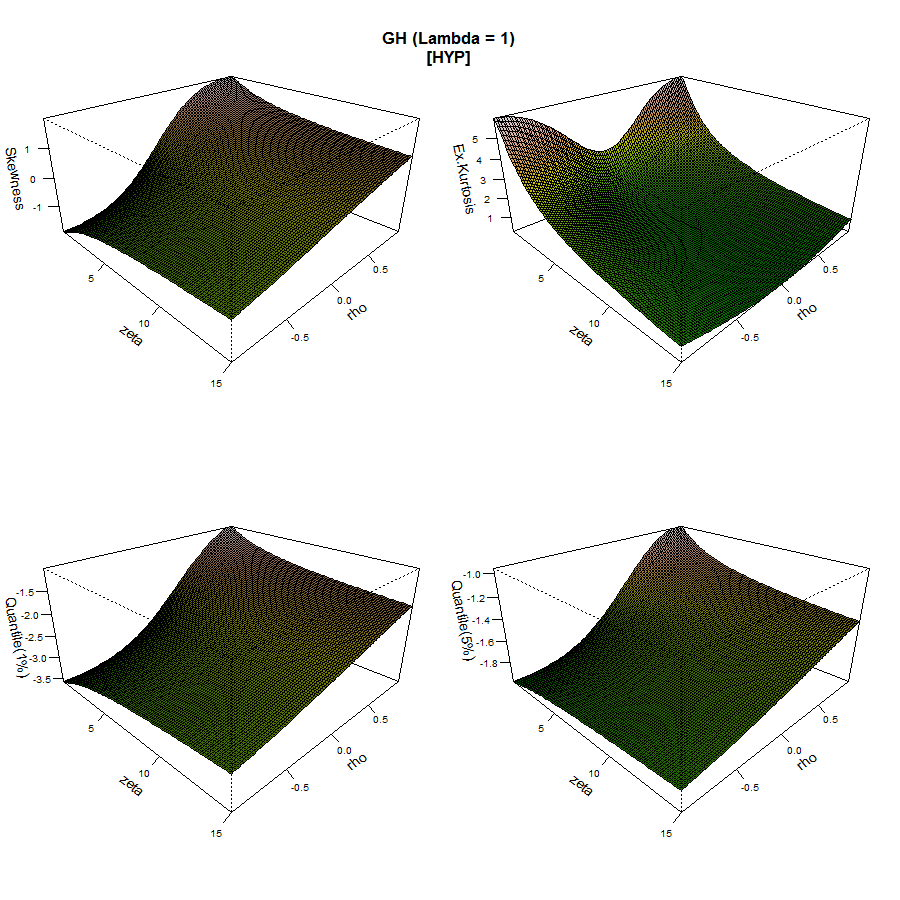
\includegraphics[scale=0.4, angle=0]{ghyp2.png}}
\subfloat[$\lambda=-0.5$(NIG)]{\label{fig:ghyp3}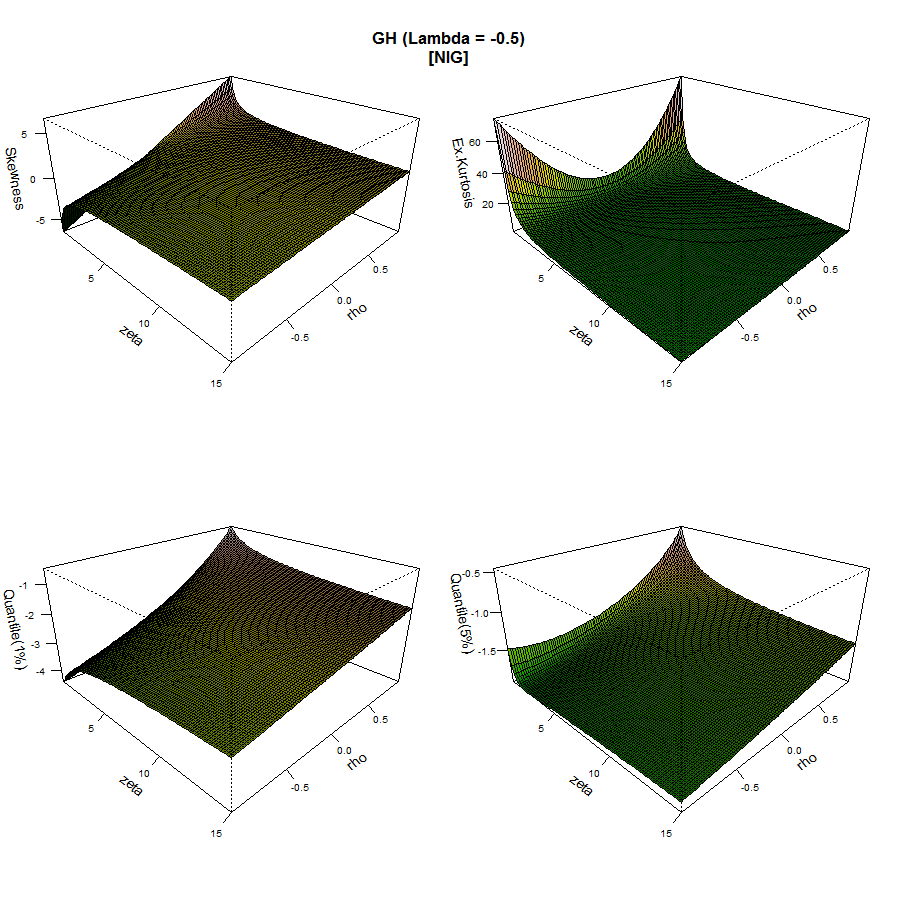
\includegraphics[scale=0.4, angle=0]{ghyp3.png}}
\caption[GH Distribution Skewness, Kurtosis and Quantile Surfaces]{GH Distribution Skewness, Kurtosis and Quantile Surfaces}\label{fig:ghsurface}
\end{figure}
\end{landscape}

\subsubsection{The Generalized Hyperbolic Skew Student Distribution}\label{ghskt}
The GH Skew-Student distribution was popularized by \cite{Aas2006} because of its uniqueness
in the GH family in having one tail with polynomial and one with exponential behavior.
This distribution is a limiting case of the GH when $\alpha  \to \left| \beta  \right|$
and $\lambda=-\nu/2$, where $\nu$ is the shape parameter of the Student distribution.
The domain of variation of the parameters is $\beta  \in \mathbb{R}$ and $\nu>0$, but
for the variance to be finite $\nu>4$, while for the existence of skewness and kurtosis,
$\nu>6$ and $\nu>8$ respectively. The density of the random variable $x$ is then given
by:
\begin{equation}
f\left( x \right) = \frac{{{2^{\left( {1 - \nu } \right)/2}}{\delta ^\nu }{{\left| \beta  \right|}^{\left( {\nu  + 1} \right)/2}}{K_{\left( {\nu  + 1} \right)/2}}\left( {\sqrt {{\beta ^2}\left( {{\delta ^2} + {{\left( {x - \mu } \right)}^2}} \right)} } \right)\exp \left( {\beta \left( {x - \mu } \right)} \right)}}
{{\Gamma \left( {\nu /2} \right)\sqrt \pi  {{\left( {\sqrt {{\delta ^2} + {{\left( {x - \mu } \right)}^2}} } \right)}^{\left( {\nu  + 1} \right)/2}}}}
\end{equation}
To standardize the distribution to have zero mean and unit variance, I make use
of the first two moment conditions for the distribution which are:
\begin{equation}
\begin{gathered}
  E\left( x \right) = \mu  + \frac{{\beta {\delta ^2}}}
{{\nu  - 2}} \hfill \\
  Var\left( x \right) = \frac{{2{\beta ^2}{\delta ^4}}}
{{{{\left( {\nu  - 2} \right)}^2}\left( {\nu  - 4} \right)}} + \frac{{{\delta ^2}}}
{{\nu  - 2}} \hfill \\
\end{gathered}
\end{equation}
We require that $Var(x)=1$, thus:
\begin{equation}
\delta  = {\left( {\frac{{2{{\bar \beta }^2}}}
{{{{\left( {\nu  - 2} \right)}^2}\left( {\nu  - 4} \right)}} + \frac{1}
{{\nu  - 2}}} \right)^{ - 1/2}}
\end{equation}
where I have made use of the $4^{th}$ parametrization of the GH distribution given in
\cite{Prause1999} where $\hat \beta = \beta \delta$. The location parameter is then rescaled
by substituting into the first moment formula $\delta$ so that it has zero mean:
\begin{equation}
\bar \mu  =  - \frac{{\beta {\delta ^2}}}{{\nu  - 2}}
\end{equation}
Therefore, we model the GH Skew-Student using the location-scale invariant parametrization $(\bar \beta, \nu)$
and then translate the parameters into the usual GH distribution's $(\alpha, \beta, \delta, \mu)$, setting
$\alpha = abs(\beta)+1e-12$.
As of version 1.2-8, the quantile function (via \textbf{qdist}) is calculated using
the SkewHyperbolic package of \cite{Scott} using the spline method (for speed), as
is the distribution function (via \textbf{pdist}).
\subsubsection{Johnson's Reparametrized SU Distribution}\label{jsu}
The reparameterized Johnson SU distribution, discussed in \cite{Rigby2005}, is a
four parameter distribution denoted by $JSU\left(\mu,\sigma,\nu,\tau\right)$,
with mean $\mu$ and standard deviation $\sigma$ for all values of the skew and
shape parameters $\nu$ and $\tau$ respectively. The implementation is taken
from the GAMLSS package of \cite{Stasinopoulos2009} and the reader is referred
there for further details.

\section{Fitting}\label{section:fitting}
Once a \verb@uGARCHspec@ has been defined, the \verb@ugarchfit@ method takes
the following arguments:
\begin{Schunk}
\begin{Sinput}
> args(ugarchfit)
\end{Sinput}
\begin{Soutput}
function (spec, data, out.sample = 0, solver = "solnp", solver.control = list(),
    fit.control = list(stationarity = 1, fixed.se = 0, scale = 0,
        rec.init = "all"), ...)
\end{Soutput}
\end{Schunk}
The out.sample option controls how many data points from the end to keep for out
of sample forecasting, while the solver.control and fit.control provide additional
options to the fitting routine. Importantly, the \emph{stationarity} option controls
whether to impose a stationarity constraint during estimation, which is usually
closely tied to the persistence of the process. The \emph{fixed.se} controls
whether, for those values which are fixed, numerical standard errors should be
calculated. The \emph{scale} option controls whether the data should be scaled prior
to estimation by its standard deviation (scaling sometimes facilitates the estimation
process). The option \emph{rec.init}, introduced in version 1.0-14 allows to set
the type of method for the conditional recursion initialization, with default
value 'all' indicating that all the data is used to calculate the mean of the
squared residuals from the conditional mean filtration. To use the first 'n' points
for the calculation, a positive integer greater than or equal to one (and less than
the total estimation datapoints) can instead be provided. If instead a positive
numeric value less than 1 is provided, this is taken as the weighting in an
exponential smoothing backcast method for calculating the initial recursion value.\\
Currently, 5 solvers \footnote{Since version $1.0-8$ the
'nlopt' solver of Johnson (interfaced to R by Jelmer Ypma in the 'nloptr' package)
has  been added, greatly expanding the range of possibilities available via its
numerous subsolver options - see documentation.} are supported, with the main
one being the augmented Lagrange solver solnp of \cite{Ye1997} implemented in R by
\cite{Ghalanos2011}.
The main functionality, namely the GARCH dynamics and conditional likelihood calculations are
done in C for speed. For reference, there is a benchmark routine called \verb@ugarchbench@
which provides a comparison of \verb@rugarch@ against 2 published GARCH models with analytic
standard errors, and a small scale comparison with a commercial GARCH implementation.
The fitted object is of class \verb@uGARCHfit@ which can be passed to a variety
of other methods such as show (summary), plot, ugarchsim, ugarchforecast etc.
The following example illustrates its use, but the interested reader should
consult the documentation on the methods available for the returned class.
\begin{Schunk}
\begin{Sinput}
> spec = ugarchspec()
> data(sp500ret)
> fit = ugarchfit(spec = spec, data = sp500ret)
> show(fit)
\end{Sinput}
\begin{Soutput}
*---------------------------------*
*          GARCH Model Fit        *
*---------------------------------*

Conditional Variance Dynamics
-----------------------------------
GARCH Model	: sGARCH(1,1)
Mean Model	: ARFIMA(1,0,1)
Distribution	: norm

Optimal Parameters
------------------------------------
        Estimate  Std. Error  t value Pr(>|t|)
mu      0.000522    0.000087   5.9873  0.00000
ar1     0.870609    0.071909  12.1070  0.00000
ma1    -0.897805    0.064324 -13.9576  0.00000
omega   0.000001    0.000001   1.3912  0.16418
alpha1  0.087714    0.013705   6.4001  0.00000
beta1   0.904955    0.013750  65.8136  0.00000

Robust Standard Errors:
        Estimate  Std. Error    t value Pr(>|t|)
mu      0.000522    0.000130   4.020100 0.000058
ar1     0.870609    0.087878   9.907060 0.000000
ma1    -0.897805    0.079989 -11.224134 0.000000
omega   0.000001    0.000014   0.093412 0.925576
alpha1  0.087714    0.186497   0.470322 0.638125
beta1   0.904955    0.191986   4.713649 0.000002

LogLikelihood : 17902.41

Information Criteria
------------------------------------

Akaike       -6.4807
Bayes        -6.4735
Shibata      -6.4807
Hannan-Quinn -6.4782

Weighted Ljung-Box Test on Standardized Residuals
------------------------------------
                        statistic   p-value
Lag[1]                      5.548 1.850e-02
Lag[2*(p+q)+(p+q)-1][5]     6.437 1.263e-05
Lag[4*(p+q)+(p+q)-1][9]     7.191 1.108e-01
d.o.f=2
H0 : No serial correlation

Weighted Ljung-Box Test on Standardized Squared Residuals
------------------------------------
                        statistic p-value
Lag[1]                      1.103  0.2935
Lag[2*(p+q)+(p+q)-1][5]     1.497  0.7407
Lag[4*(p+q)+(p+q)-1][9]     1.956  0.9102
d.o.f=2

Weighted ARCH LM Tests
------------------------------------
            Statistic Shape Scale P-Value
ARCH Lag[3]   0.01965 0.500 2.000  0.8885
ARCH Lag[5]   0.17504 1.440 1.667  0.9713
ARCH Lag[7]   0.53718 2.315 1.543  0.9749

Nyblom stability test
------------------------------------
Joint Statistic:  174.6662
Individual Statistics:
mu      0.2090
ar1     0.1488
ma1     0.1057
omega  21.3780
alpha1  0.1345
beta1   0.1130

Asymptotic Critical Values (10% 5% 1%)
Joint Statistic:     	 1.49 1.68 2.12
Individual Statistic:	 0.35 0.47 0.75

Sign Bias Test
------------------------------------
                   t-value      prob sig
Sign Bias           0.4298 6.674e-01
Negative Sign Bias  2.9478 3.214e-03 ***
Positive Sign Bias  2.3929 1.675e-02  **
Joint Effect       28.9794 2.262e-06 ***


Adjusted Pearson Goodness-of-Fit Test:
------------------------------------
  group statistic p-value(g-1)
1    20     179.0    4.951e-28
2    30     188.1    3.195e-25
3    40     218.6    7.737e-27
4    50     227.6    7.927e-25


Elapsed time : 1.295898
\end{Soutput}
\end{Schunk}

\subsection{Fit Diagnostics}\label{section:diagnostics}
The summary method for the \verb@uGARCHfit@ object provides the parameters and
their standard errors (and a robust version), together with a variety of tests
which can also be called individually.\\
The robust standard errors are based on the method of \cite{White1982} which produces
asymptotically valid confidence intervals by calculating the covariance ($V$) of the
parameters $(\theta)$ as:
\begin{equation}
\hat V =  {\left( -A \right)^{ - 1}}B{\left( { - A} \right)^{ - 1}}
\end{equation}
where,
\begin{equation}
\begin{gathered}
  A = L''\left( {\hat \theta } \right) \hfill \\
  B = {\sum\limits_{i = 1}^n {{g_i}\left( {{x_i}\left| {\hat \theta } \right.} \right)} ^T}{g_i}\left( {{x_i}\left| {\hat \theta } \right.} \right) \hfill \\
\end{gathered}
\end{equation}
which is the Hessian and covariance of the scores at the optimum.
The robust standard errors are the square roots of the diagonal of $V$.\\
The \verb@inforcriteria@ method on a fitted or filtered object returns the
Akaike (AIC), Bayesian (BIC), Hannan-Quinn (HQIC) and Shibata (SIC) information
criteria to enable model selection by penalizing overfitting at different rates.
Formally, they may be defined as:
\begin{equation}\label{inforcriteria}
\begin{gathered}
  AIC = \frac{{ - 2LL}}
{N} + \frac{{2m}}
{N} \hfill \\
  BIC = \frac{{ - 2LL}}
{N} + \frac{{m{{\log }_e}\left( N \right)}}
{N} \hfill \\
  HQIC = \frac{{ - 2LL}}
{N} + \frac{{\left( {2m{{\log }_e}\left( {{{\log }_e}\left( N \right)} \right)} \right)}}
{N} \hfill \\
  SIC = \frac{{ - 2LL}}
{N} + {\log _e}\left( {\frac{{\left( {N + 2m} \right)}}
{N}} \right) \hfill \\
\end{gathered}
\end{equation}
were any parameters fixed during estimation are excluded from the calculation.
Since version 1.3-1, the Q-statistics and ARCH-LM test have been replaced with the
Weighted Ljung-Box and ARCH-LM statistics of \cite{Fisher2012a} which better account
for the distribution of the statistics of the values from the estimated models.
The ARCH-LM test is now a weighted portmanteau test for testing the null hypothesis
of adequately fitted ARCH process, whilst the Ljung-Box is another portmanteau test
with null the adequacy of the ARMA fit.
The \verb@signbias@ calculates the Sign Bias Test of \cite{Engle1993}, and is also
displayed in the summary. This tests the presence of leverage effects in the
standardized residuals (to capture possible misspecification of the GARCH model),
by regressing the squared standardized residuals on lagged negative and positive
shocks as follows:
\begin{equation}\label{signbias}
\hat z_t^2 = {c_0} + {c_1}{I_{{{\hat \varepsilon}_{t - 1}} < 0}} +
{c_2}{I_{{{\hat \varepsilon}_{t - 1}} < 0}}{\hat \varepsilon_{t - 1}} + {c_3}{I_{{{\hat \varepsilon}_{t - 1}} \geqslant 0}}{\hat \varepsilon_{t - 1}} + {u_t}
\end{equation}
where $I$ is the indicator function and $\hat \varepsilon_t$ the estimated residuals
from the GARCH process. The Null Hypotheses are $H_0:c_i=0$ (for $i=1,2,3$), and that
jointly $H_0:c_1=c_2=c_3=0$. As can be inferred from the summary of the previous
fit, there is significant Negative and Positive reaction to shocks. Using
instead a model such as the apARCH would likely alleviate these effects.

The \verb@gof@ calculates the chi-squared goodness of fit test, which compares
the empirical distribution of the standardized residuals with the theoretical
ones from the chosen density. The implementation is based on the test of
\cite{Palm1996} which adjusts the tests in the presence on non-i.i.d. observations
by reclassifying the standardized residuals not according to their value (as in
the standard test), but instead on their magnitude, calculating the probability
of observing a value smaller than the standardized residual, which should be
identically standard uniform distributed. The function must take 2 arguments, the
fitted object as well as the number of bins to classify the values. In the
summary to the fit, a choice of $(20,30,40,50)$ bins is used, and from the
summary of the previous example it is clear that the Normal distribution does
not adequately capture the empirical distribution based on this test.

The \verb@nymblom@ test calculates the parameter stability test of \cite{Nyblom1989},
as well as the joint test. Critical values against which to compare the results
are displayed, but this is not available for the joint test in the case of more than 20
parameters.

Finally, some informative plots can be drawn either interactively(which = 'ask'),
individually (which = 1:12) else all at once (which = 'all') as in Figure
\ref{fig:fitplot}.

\begin{landscape}
\begin{figure}[!ht]
\centering
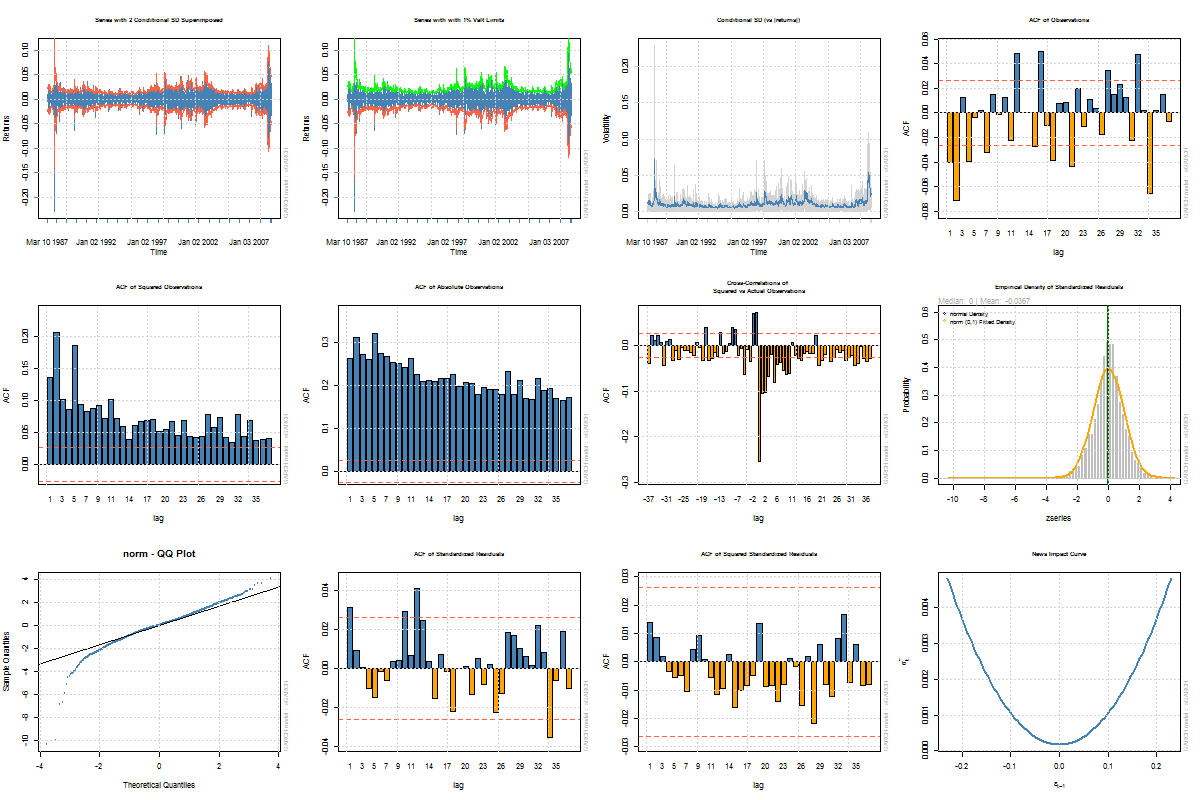
\includegraphics[width=22cm]{fitplot.png}
\caption[uGARCHfit Plots]{uGARCHfit Plots}\label{fig:fitplot}
\end{figure}
\end{landscape}

\section{Filtering}\label{section:filtering}
Sometimes it is desirable to simply filter a set of data with a predefined set
of parameters. This may for example be the case when new data has arrived and
one might not wish to re-fit. The \verb@ugarchfilter@ method does exactly that,
taking a \verb@uGARCHspec@ object with fixed parameters. Setting fixed or
starting parameters on the GARCH spec object may be done either through the
\verb@ugarchspec@ function when it is called via the fixed.pars arguments to the
function, else by using the \verb@setfixed<-@ method on the spec object.
The example which follows explains how:
\begin{Schunk}
\begin{Sinput}
> data(sp500ret)
> spec = ugarchspec(variance.model = list(model = "apARCH"), distribution.model = "std")
> setfixed(spec) <- list(mu = 0.01, ma1 = 0.2, ar1 = 0.5, omega = 1e-05,
+     alpha1 = 0.03, beta1 = 0.9, gamma1 = 0.01, delta = 1, shape = 5)
> filt = ugarchfilter(spec = spec, data = sp500ret)
> show(filt)
\end{Sinput}
\begin{Soutput}
*------------------------------------*
*          GARCH Model Filter        *
*------------------------------------*

Conditional Variance Dynamics
--------------------------------------
GARCH Model	: apARCH(1,1)
Mean Model	: ARFIMA(1,0,1)
Distribution	: std

Filter Parameters
---------------------------------------

mu     1e-02
ar1    5e-01
ma1    2e-01
omega  1e-05
alpha1 3e-02
beta1  9e-01
gamma1 1e-02
delta  1e+00
shape  5e+00

LogLikelihood : 5627.392

Information Criteria
---------------------------------------

Akaike       -2.0378
Bayes        -2.0378
Shibata      -2.0378
Hannan-Quinn -2.0378

Weighted Ljung-Box Test on Standardized Residuals
---------------------------------------
                        statistic p-value
Lag[1]                       1178       0
Lag[2*(p+q)+(p+q)-1][5]      1212       0
Lag[4*(p+q)+(p+q)-1][9]      1217       0
d.o.f=2
H0 : No serial correlation

Weighted Ljung-Box Test on Standardized Squared Residuals
---------------------------------------
                        statistic p-value
Lag[1]                      170.4       0
Lag[2*(p+q)+(p+q)-1][5]     173.8       0
Lag[4*(p+q)+(p+q)-1][9]     175.8       0
d.o.f=2

Weighted ARCH LM Tests
---------------------------------------
            Statistic Shape Scale P-Value
ARCH Lag[3]     3.915 0.500 2.000 0.04785
ARCH Lag[5]     4.207 1.440 1.667 0.15612
ARCH Lag[7]     5.237 2.315 1.543 0.20163


Sign Bias Test
---------------------------------------
                   t-value      prob sig
Sign Bias           8.3144 1.150e-16 ***
Negative Sign Bias  5.6999 1.261e-08 ***
Positive Sign Bias  0.5621 5.741e-01
Joint Effect       95.8328 1.223e-20 ***


Adjusted Pearson Goodness-of-Fit Test:
---------------------------------------
  group statistic p-value(g-1)
1    20     86296            0
2    30    128891            0
3    40    169014            0
4    50    207506            0
\end{Soutput}
\end{Schunk}
The returned object is of class \verb@uGARCHfilter@ and shares many of the methods
as the \verb@uGARCHfit@ class. Additional arguments to the function are explained
in the documentation. Note that the information criteria shown here are based on
zero estimated parameters (they are all fixed), and the same goes for the
\emph{infocriteria} method on a \verb@uGARCHfilter@ object.

\section{Forecasting and the GARCH Bootstrap}\label{section:forecasting}
There are 2 types of forecasts available with the package. A rolling method,
whereby consecutive 1-ahead forecasts are created based on the out.sample option
set in the fitting routine, and an unconditional method for n>1 ahead forecasts.
(and it is also possible to combine the 2 creating a rather complicated object).
In the latter case, it is also possible to make use of the GARCH bootstrap,
described in \cite{Pascual2006} and implemented in the function \verb@ugarchboot@,
with the added innovation of an optional extra  step of fitting either a kernel
or semi-parametric density (SPD) to the standardized residuals prior to sampling
in order to provide for (possibly) more robustness  in the presence of limited data.
To understand what the GARCH bootstrap does, consider that there are two main
sources of uncertainty about n.ahead forecasting from GARCH models: that arising
from the form of the predictive density and that due to parameter uncertainty.
The bootstrap method in the \verb@rugarch@ package is based on
resampling standardized residuals from the empirical distribution of the fitted model
to generate future realizations of the series and sigma. Two methods are implemented:
one takes into account parameter uncertainty by building a simulated distribution
of the parameters through simulation and refitting, and one which only considers
distributional uncertainty and hence avoids the expensive and lengthy parameter
distribution estimation. In the latter case, prediction intervals for the 1-ahead sigma
forecast will not be available since only the parameter uncertainty is relevant in
GARCH type models in this case. The following example provides for a brief look at the
partial method, but the interested reader should consult the more comprehensive examples
in the inst folder of the package.
\begin{Schunk}
\begin{Sinput}
> data(sp500ret)
> spec = ugarchspec(variance.model=list(model="csGARCH"), distribution="std")
> fit = ugarchfit(spec, sp500ret)
> bootp = ugarchboot(fit, method = c("Partial", "Full")[1],
+ n.ahead = 500, n.bootpred = 500)
> show(bootp)
\end{Sinput}
\begin{Soutput}
*-----------------------------------*
*     GARCH Bootstrap Forecast      *
*-----------------------------------*
Model : csGARCH
n.ahead : 500
Bootstrap method:  partial
Date (T[0]): 2009-01-30

Series (summary):
          min      q.25      mean     q.75      max forecast[analytic]
t+1  -0.10855 -0.013343  0.000668 0.016285 0.090454           0.001944
t+2  -0.11365 -0.010796  0.001632 0.015721 0.085783           0.001707
t+3  -0.28139 -0.013203 -0.000378 0.015496 0.082250           0.001512
t+4  -0.10459 -0.014830  0.000346 0.015602 0.109223           0.001352
t+5  -0.21915 -0.012494  0.001196 0.016627 0.098003           0.001220
t+6  -0.11029 -0.012119  0.001008 0.015000 0.083469           0.001112
t+7  -0.22818 -0.013280  0.000398 0.015250 0.094184           0.001023
t+8  -0.25722 -0.014854 -0.001401 0.016074 0.088067           0.000949
t+9  -0.34629 -0.017681 -0.004484 0.012847 0.154058           0.000889
t+10 -0.11328 -0.013566  0.000957 0.018291 0.140734           0.000840
.....................

Sigma (summary):
          min    q0.25     mean    q0.75      max forecast[analytic]
t+1  0.026387 0.026387 0.026387 0.026387 0.026387           0.026387
t+2  0.025518 0.025564 0.026345 0.026493 0.038492           0.026577
t+3  0.024698 0.025021 0.026332 0.026768 0.039903           0.026614
t+4  0.023925 0.024682 0.026440 0.027087 0.077525           0.026649
t+5  0.023259 0.024456 0.026474 0.027507 0.074919           0.026682
t+6  0.022622 0.024173 0.026498 0.027687 0.072876           0.026714
t+7  0.021988 0.023855 0.026463 0.027700 0.069719           0.026744
t+8  0.021503 0.023684 0.026424 0.027785 0.070750           0.026772
t+9  0.021044 0.023677 0.026690 0.028065 0.071725           0.026799
t+10 0.020560 0.023589 0.027050 0.028363 0.095243           0.026824
.....................

\end{Soutput}
\end{Schunk}
\begin{figure}
\centering
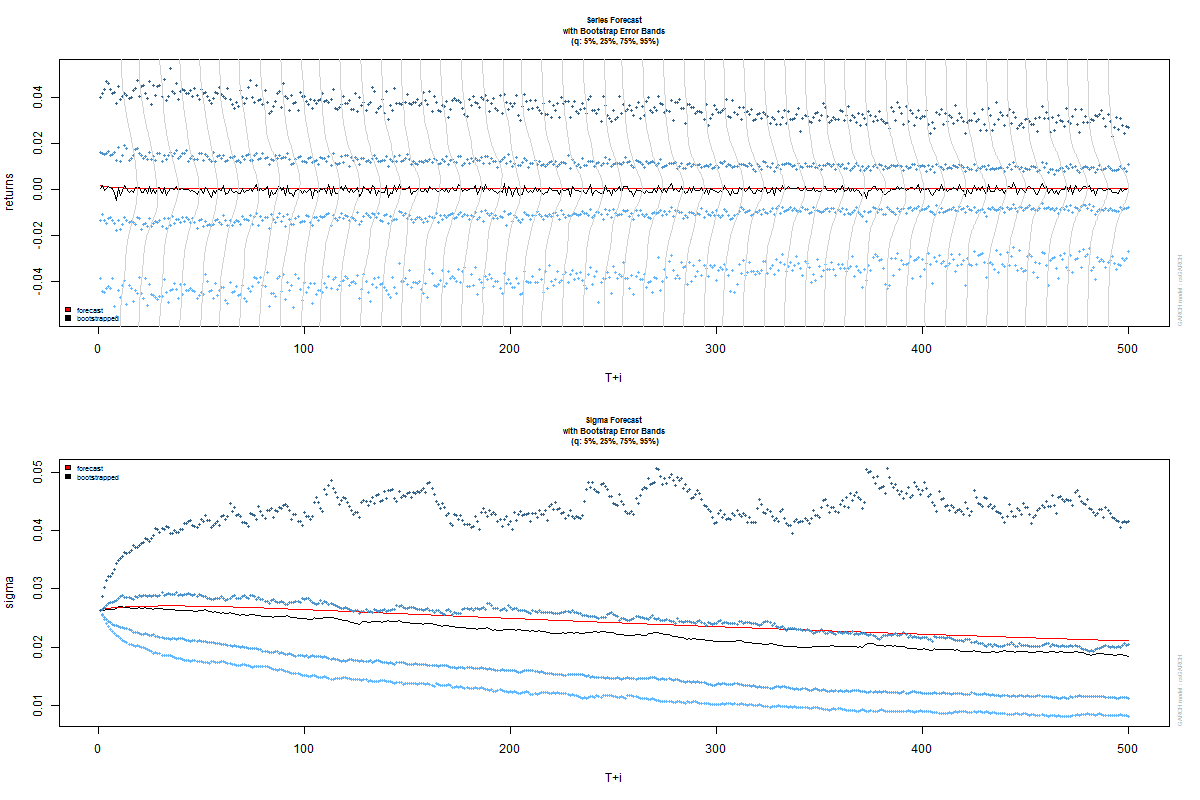
\includegraphics{boot_partial.png}
\caption[GARCH Bootstrap Forecast Plots]{GARCH Bootstrap Forecast Plots}\label{fig:bootplot}
\end{figure}
The 'recipe' for the full GARCH bootstrap is summarized below:
\begin{enumerate}
\item Extract the standardized residuals from the estimated object. If it is a specification with
fixed parameters, first filter using the supplied dataset and then extract the standardized
residuals from the filtered object.
\item Sample n.bootfit sets of size N (original dataset less any out of sample periods) from either
the raw standardized residuals, using the spd or kernel based methods.
\item Simulate n.bootfit paths of size N, using as innovations the sampled standardized residuals. The
simulation is initiated with the last values from the dataset at point N ($T_0$ in simulation time).
\item The n.bootfit simulated series are then estimated with the same specification used by the originally
supplied object in order to generate a set of coefficients representing the parameter uncertainty.
\item Filter the original dataset with the n.bootfit set of estimated coefficients.
\item Use the last values of the filtered conditional sigma (and if it is the csGARCH model, then also the
permanent component q) and residuals from the previous step to initialize a new simulation with horizon
n.ahead and m.sim=n.bootpred, using again the standardized residuals sampled as in step 2 and the new set of
estimated coefficients. The simulation now contains uncertainty about the conditional n-ahead density as well
as parameter uncertainty.
\end{enumerate}
\section{Simulation}\label{section:simulation}
Simulation may be carried out either directly on a fitted object (\verb@ugarchsim@)
else on a GARCH spec with fixed parameters (\verb@ugarchpath@). The \verb@ugarchsim@
method takes the following arguments:
\begin{Schunk}
\begin{Sinput}
> args(ugarchsim)
\end{Sinput}
\begin{Soutput}
function (fit, n.sim = 1000, n.start = 0, m.sim = 1, startMethod = c("unconditional",
    "sample"), presigma = NA, prereturns = NA, preresiduals = NA,
    rseed = NA, custom.dist = list(name = NA, distfit = NA),
    mexsimdata = NULL, vexsimdata = NULL, ...)
\end{Soutput}
\end{Schunk}
where the n.sim indicates the length of the simulation while m.sim the number of
independent simulations. For reasons of speed, when n.sim is large relative to
m.sim, the simulation code is executed in C, while for large m.sim a special
purpose C++ code (using Rcpp and RcppArmadillo) is used which was found to lead
to significant speed increase. Key to replicating results is the rseed argument
which is used to pass a user seed to initialize the random number generator, else
one will be assigned by the program. In any case, the returned object, of class
\verb@uGARCHsim@ (or \verb@uGARCHpath@) contains a slot with the seed(s) used.
\section{Rolling Estimation}\label{section:rolling}
The \verb@ugarchroll@ method allows to perform a rolling estimation and
forecasting of a model/dataset combination, optionally returning the VaR at
specified levels. More importantly, it returns the distributional forecast
parameters necessary to calculate any required measure on the forecasted
density. The following example illustrates the use of the method where use is
also made of the parallel functionality and run on 10 cores.\footnote{\textbf{Since version 1.0-14
the parallel functionality is based on the paralllel package and it is upto the
user to initialize a cluster object and pass it to the function, and then terminate
it once it is no longer required. Eventually, this approach to the parallel usage
will filter through to all the functions in rugarch and rmgarch.}}
Figure \ref{fig:roll} is generated by calling the plot function on the
returned \verb@uGARCHroll@ object. Additional methods, and more importantly
extractor functions can be found in the documentation. \textbf{Note that only n.ahead=1 is allowed at
present (more complicated rolling forecasts can be created by the user with
the ugarchfit and ugarchforecast functions).} Finally, there is a new method
called \emph{resume} which allows resumption of estimation of an object which had
non-converged windows, optionally supplying a different solver and solver control
combination.
\begin{Schunk}
\begin{Sinput}
> data(sp500ret)
> library(parallel)
> cl = makePSOCKcluster(10)
> spec = ugarchspec(variance.model = list(model = "eGARCH"), distribution.model = "jsu")
> roll = ugarchroll(spec, sp500ret, n.start = 1000, refit.every = 100,
refit.window = "moving", solver = "hybrid", calculate.VaR = TRUE,
VaR.alpha = c(0.01, 0.05), cluster = cl, keep.coef = TRUE)
>show(roll)
>stopCluster(cl)
\end{Sinput}
\begin{Soutput}
*-------------------------------------*
*              GARCH Roll             *
*-------------------------------------*
No.Refits       : 46
Refit Horizon   : 100
No.Forecasts    : 4523
GARCH Model     : eGARCH(1,1)
Distribution    : jsu

Forecast Density:
              Mu  Sigma    Skew  Shape Shape(GIG) Realized
1991-02-21 4e-04 0.0102 -0.2586 1.5065          0  -0.0005
1991-02-22 2e-04 0.0099 -0.2586 1.5065          0   0.0019
1991-02-25 4e-04 0.0095 -0.2586 1.5065          0   0.0044
1991-02-26 3e-04 0.0093 -0.2586 1.5065          0  -0.0122
1991-02-27 1e-04 0.0101 -0.2586 1.5065          0   0.0135
1991-02-28 7e-04 0.0099 -0.2586 1.5065          0  -0.0018

..........................
                Mu  Sigma  Skew Shape Shape(GIG) Realized
2009-01-23  0.0015 0.0259 -0.87 2.133          0   0.0054
2009-01-26  0.0005 0.0243 -0.87 2.133          0   0.0055
2009-01-27 -0.0002 0.0228 -0.87 2.133          0   0.0109
2009-01-28 -0.0011 0.0212 -0.87 2.133          0   0.0330
2009-01-29 -0.0039 0.0191 -0.87 2.133          0  -0.0337
2009-01-30  0.0009 0.0220 -0.87 2.133          0  -0.0231

Elapsed: 12.97949 secs
\end{Soutput}
\begin{Sinput}
> report(roll, type = "VaR", VaR.alpha = 0.05, conf.level = 0.95)
\end{Sinput}
\begin{Soutput}
VaR Backtest Report
===========================================
Model:                  eGARCH-jsu
Backtest Length:        4523
==========================================
alpha:                  5%
Expected Exceed:        226.2
Actual VaR Exceed:      253
Actual %:               5.6%

Unconditional Coverage (Kupiec)
Null-Hypothesis:        Correct Exceedances
LR.uc Statistic:        0
LR.uc Critical:         3.841
LR.uc p-value:          1
Reject Null:            NO

Conditional Coverage (Christoffersen)
Null-Hypothesis:        Correct Exceedances and
                        Independence of Failures
LR.cc Statistic:        0
LR.cc Critical:         5.991
LR.cc p-value:          1
Reject Null:            NO
\end{Soutput}
\end{Schunk}
\begin{figure}
\centering
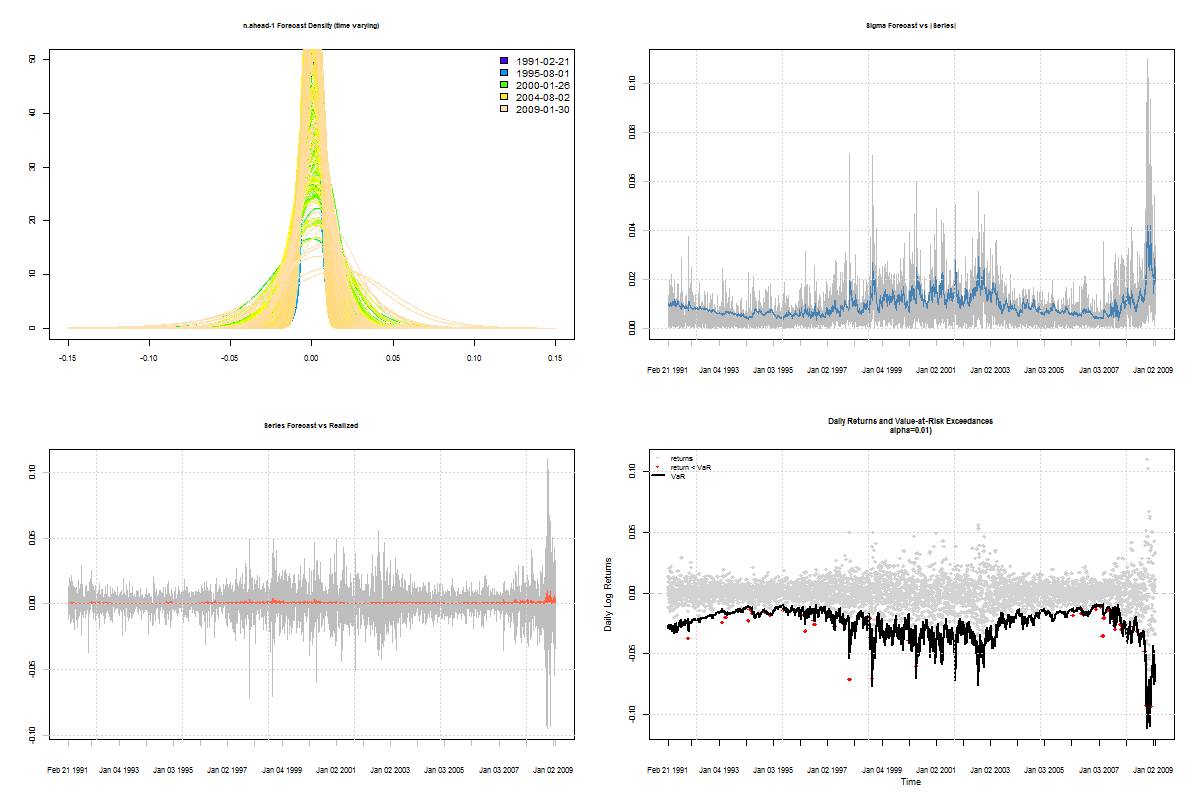
\includegraphics{roll.png}
\caption[eGARCH Rolling Forecast Plots]{eGARCH Rolling Forecast Plots}\label{fig:roll}
\end{figure}
\clearpage
\section{Simulated Parameter Distribution and RMSE}\label{section:ugarchdist}
It is sometimes instructive to be able to investigate the underlying
density of the estimated parameters under different models. The \verb@ugarchdistribution@
method performs a monte carlo experiment by simulating and fitting a model
multiple times and for different 'window' sizes. This allows to obtain some insight
on the consistency of the parameter estimates as the data window increases by
looking at the rate of decrease of the Root Mean Squared Error and whether we
have $\sqrt N$ consistency. This is a computationally expensive exercise and as
such should only be undertaken in the presence of ample computing power and RAM.
As in other functions, parallel functionality is enabled if available.
The example which follows illustrates an instance of this test on one model and
one set of parameters. Figures \ref{fig:dist1} and \ref{fig:dist2} complete this
example.
\begin{Schunk}
\begin{Sinput}
> spec = ugarchspec(variance.model = list(model = "gjrGARCH"),
+     distribution.model = "ged")
> print(persistence(pars = unlist(list(mu = 0.001, ar1 = 0.4, ma1 = -0.1,
+     omega = 1e-06, alpha1 = 0.05, beta1 = 0.9, gamma1 = 0.05,
+     shape = 1.5)), distribution = "ged", model = "gjrGARCH"))
\end{Sinput}
\begin{Soutput}
persistence
      0.975
\end{Soutput}
\begin{Sinput}
> library(parallel)
> cl = makePSOCKcluster(10)
> setfixed(spec) <- list(mu = 0.001, ar1 = 0.4, ma1 = -0.1, omega = 1e-06,
+     alpha1 = 0.05, beta1 = 0.9, gamma1 = 0.05, shape = 1.5)
> dist = ugarchdistribution(fitORspec = spec, n.sim = 2000, n.start = 1,
+     m.sim = 100, recursive = TRUE, recursive.length = 6000, recursive.window = 1000,
+     rseed = 1066, solver = "solnp", solver.control = list(trace = 0),
+     cluster = cl)
> stopCluster(cl)
> show(dist)
\end{Sinput}
\begin{Soutput}
*------------------------------------*
*    GARCH Parameter Distribution    *
*------------------------------------*
Model : gjrGARCH
No. Paths (m.sim) : 100
Length of Paths (n.sim) : 2000
Recursive : TRUE
Recursive Length : 6000
Recursive Window : 1000

Coefficients: True vs Simulation Mean (Window-n)
                    mu     ar1       ma1      omega   alpha1   beta1   gamma1  shape
true-coef   0.00100000 0.40000 -0.100000 1.0000e-06 0.050000 0.90000 0.050000 1.5000
window-2000 0.00097099 0.39679 -0.097585 1.0411e-06 0.046161 0.90177 0.051709 1.4945
window-3000 0.00101520 0.38907 -0.089494 9.9344e-07 0.046741 0.90192 0.052902 1.4957
window-4000 0.00099876 0.39329 -0.094523 9.9556e-07 0.049385 0.90179 0.047515 1.4924
window-5000 0.00099491 0.40223 -0.103767 9.7545e-07 0.048651 0.90220 0.049442 1.4900
window-6000 0.00098876 0.39540 -0.096411 9.8975e-07 0.048753 0.90096 0.050907 1.4901
\end{Soutput}
\end{Schunk}
\begin{landscape}
\begin{figure}[!ht]
\centering
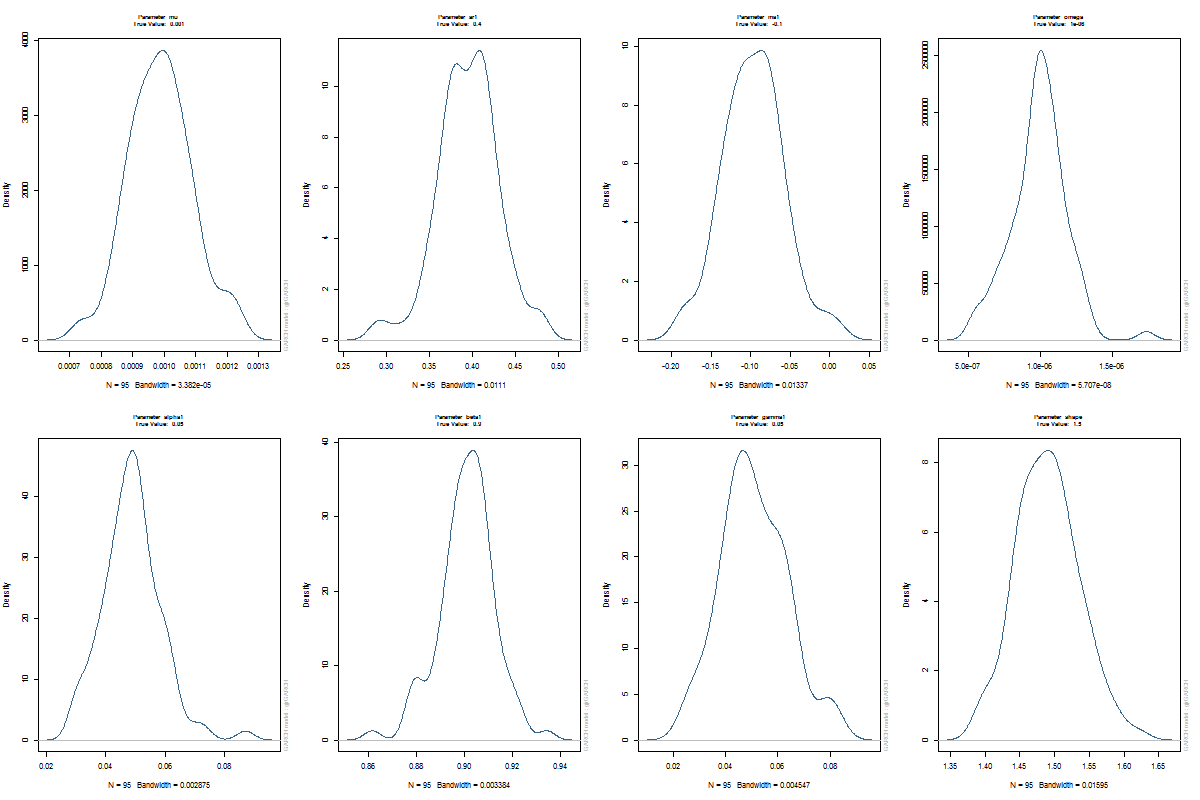
\includegraphics[width=22cm]{dist1.png}
\caption[GARCH Simulated Parameters Density]{Simulated Parameter Density}\label{fig:dist1}
\end{figure}
\begin{figure}[!ht]
\centering
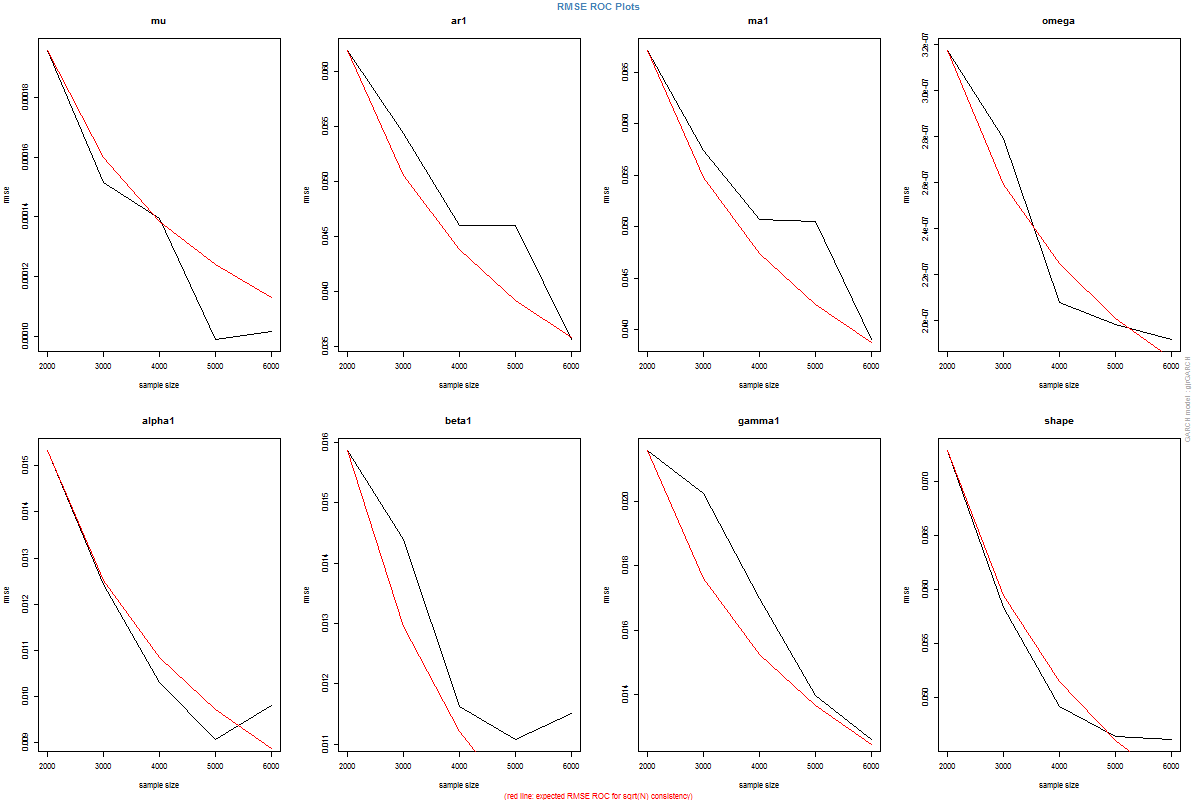
\includegraphics[width=22cm]{dist11.png}
\caption[GARCH Parameters RMSE Rate of Change]{RMSE Rate of Change}\label{fig:dist2}
\end{figure}
\begin{figure}[!ht]
\centering
\subfloat[Bivariate Parameter Plots]{\label{fig:dist3}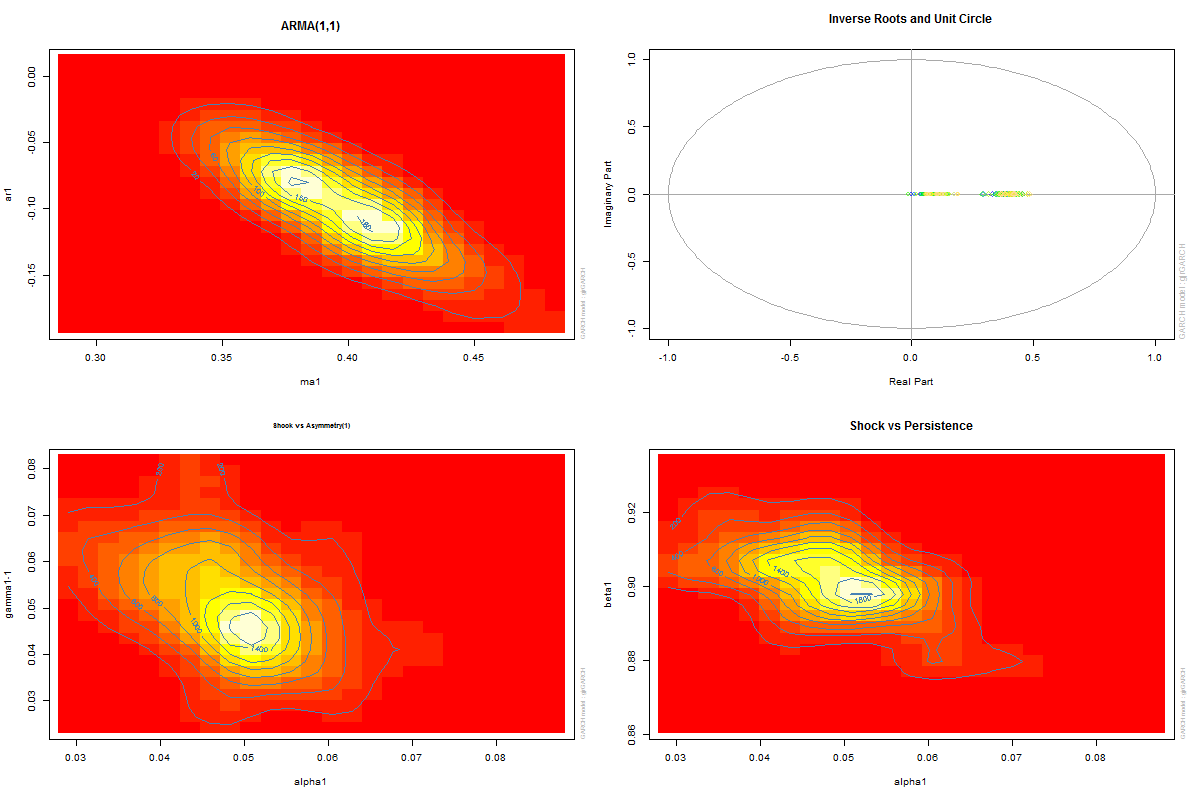
\includegraphics[scale=0.4, angle=0]{dist2.png}}
\subfloat[GARCH Stat Plots]{\label{fig:dist4}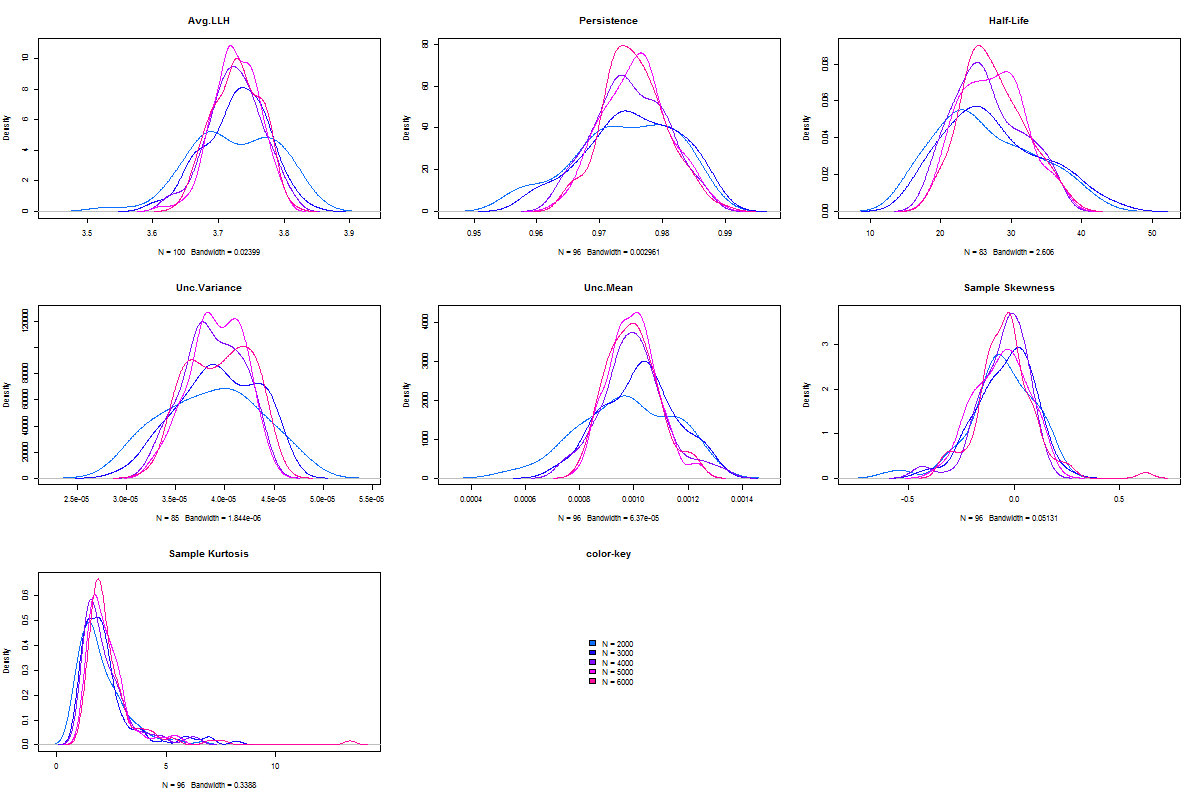
\includegraphics[scale=0.4, angle=0]{dist3.png}}
\caption[GARCH Simulated Parameters Density]{GARCH Simulated Parameters Density}\label{fig:dist3}
\end{figure}
\end{landscape}
\section{The ARFIMAX Model with constant variance}\label{section:arfima}
The \verb@rugarch@ package implements an additional set of methods and classes,
mirroring those of the GARCH specification, for modelling ARFIMAX processes
with constant variance via Maximum Likelihood. With the exception of plots, the
functionality is very similar to that covered so far for GARCH methods. The main
functions are \verb@arfimaspec@, \verb@arfimafit@, \verb@arfimaforecast@,
\verb@arfimasim@, \verb@arfimapath@, \verb@arfimadistirbution@ and \verb@arfimaroll@.
The usual extractor, inference and summary methods are replicated for all the
ARFIMA classes and the user should consult the documentation for further details.

\section{Mispecification and Other Tests}
Apart from the usual tests presented in the summary to the fit object, a number
of other interesting and useful tests are uniquely implemented in the \verb@rugarch@
package, and described in this section.
\subsection{The GMM Orthogonality Test}
The GMM type moment (orthogonality) tests of \cite{Hansen1982} have been applied
to test the adequacy of model in a variety of setups. Under a correctly
specified model, certain population moment conditions should be satisfied and
hold in the sample using the standardized residuals. The moment conditions can
be tested both individually using a t-test or jointly using a Wald test. Formally,
the following moment conditions are tested:
\begin{equation}\label{eq:gmm}
\begin{array}{*{20}{c}}
{{M_1}}&{E\left[ {{z_t}} \right]}&{ = 0}\\
{{M_2}}&{E\left[ {z_t^2 - 1} \right]}&{ = 0}\\
{{M_3}}&{E\left[ {z_t^3} \right]}&{ = 0}\\
{{M_4}}&{E\left[ {z_t^4 - 3} \right]}&{ = 0}\\
{{Q_2}}&{E\left[ {\left( {z_t^2 - 1} \right)\left( {z_{t - j}^2 - 1} \right)} \right]}&{ = 0}\\
{{Q_3}}&{E\left[ {\left( {z_t^3} \right)\left( {z_{t - j}^3} \right)} \right]}&{ = 0}\\
{{Q_4}}&{E\left[ {\left( {z_t^4 - 3} \right)\left( {z_{t - j}^4 - 3} \right)} \right]}&{ = 0}\\
\end{array}
\end{equation}
where $j=1\dots,p$ is the lag (defaults to 4 in the function), $M_1$ to $M_4$ denotes the individual moment conditions (t-test),
and $Q_2$ to $Q_4$ the joint conditional moment conditions (variance, skewness and kurtosis) which are distributed $\chi^2$ with $p$ d.o.f. All the
moment conditions can also be tested jointly using a Wald test distributed $\chi^2$ with $3p+4$ d.o.f. The test is implemented under the name: \verb@GMMTest@.
\subsection{Parametric and Non-Parametric Density Tests}
A novel method to analyze how well a conditional density fits the underlying data
is through the probability integral transformation (\emph{PIT}) discussed in
\cite{Rosenblatt1952} and defined as:
\begin{equation}
{x_t} = \int\limits_{ - \infty }^{{y_t}} {\hat f\left( u \right)du = \hat F\left( {{y_t}} \right)}
\end{equation}
which transforms the data $y_t$, using the estimated distribution $\hat F$ into
i.i.d. $U(0,1)$ under the correctly specified model. Based on this transformation,
\cite{Tay1998} provide for a visual assessment test, while \cite{Berkowitz2001}
provides a more formal test, implemented in the package under the name \verb@BerkowitzTest@.
Because of the difficulty in testing a $U(0,1)$ sequence, the PIT data is
transformed into $N(0,1)$ by Berkowitz using the normal quantile function, and
tested using a Lagrange Multiplier (\emph{LM}) test for any residual
autocorrelation given a specified number of lags. In addition, a tail
test based on the censored Normal is also provided, under the Null that the
standardized tail data has mean zero and unit variance. More recently,
\cite{Hong2005} introduced a nonparametric portmanteau test, building on the work
of \cite{Ait-Sahalia1996}, which tests the joint hypothesis of i.i.d \emph{AND} $U(0,1)$
for the sequence $x_t$. As noted by the authors, testing $x_t$ using a standard
goodness-of-fit test (such as the Kolmogorov-Smirnov) would only check the $U(0,1)$
assumption under i.i.d. and not the joint assumption of $U(0,1)$ and i.i.d. Their
approach is to compare a kernel estimator $\hat g_j\left(x_1,x_2\right)$ for the
joint density $g_j\left(x_1,x_2\right)$ of the pair  $\left\{ {x_t,x_{t-j}} \right\}$
(where $j$ is the lag order) with unity, the product of two $U(0,1)$ densities.
Given a sample size $n$ and lag order $j>0$, their joint density estimator is:
\begin{equation}\label{eq:HL1}
{{\hat g}_j}\left( {{x_1},{x_2}} \right) \equiv {\left( {n - j} \right)^{ - 1}}\sum\limits_{t = j + 1}^n {{K_h}\left( {{x_1},{{\hat X}_t}} \right){K_h}\left( {{x_2},{{\hat X}_{t - j}}} \right)}
\end{equation}
where ${{\hat X}_t} = {X_t}\left( {\hat \theta } \right)$, and $\hat \theta$ is a $\sqrt n$ consistent estimator of $\theta_0$. The function $K_h$ is a boundary
modified kernel defined as:
\begin{equation}\label{eq:HL2}
{K_h}\left( {x,y} \right) \equiv \left\{ {\begin{array}{*{20}{c}}
{{{{h^{ - 1}}k\left( {\frac{{x - y}}{h}} \right)} \mathord{\left/
 {\vphantom {{{h^{ - 1}}k\left( {\frac{{x - y}}{h}} \right)} {\int_{ - \left( {x/h} \right)}^1 {k\left( u \right)du} ,}}} \right.
 \kern-\nulldelimiterspace} {\int_{ - \left( {x/h} \right)}^1 {k\left( u \right)du} ,}}}&{{\rm{if }}x \in \left[ {0,h} \right),}\\
{{h^{ - 1}}k\left( {\frac{{x - y}}{h}} \right),}&{{\rm{if }}x \in \left[ {h,1 - h} \right],}\\
{{{{h^{ - 1}}k\left( {\frac{{x - y}}{h}} \right)} \mathord{\left/
 {\vphantom {{{h^{ - 1}}k\left( {\frac{{x - y}}{h}} \right)} {\int_{ - 1}^{\left( {1 - x} \right)/h} {k\left( u \right)du} ,}}} \right.
 \kern-\nulldelimiterspace} {\int_{ - 1}^{\left( {1 - x} \right)/h} {k\left( u \right)du} ,}}}&{{\rm{if }}x \in \left( {1 - h,1} \right],}
\end{array}} \right.
\end{equation}
where $h\equiv h\left(n \right)$ is a bandwidth such that $h\rightarrow 0$ as $n\rightarrow \infty$, and the kernel $k(.)$ is a pre-specified symmetric probability density, which is implemented as suggested by the authors using a quartic kernel,
\begin{equation}\label{eq:quartic}
k\left( u \right) = \frac{{15}}{{16}}{\left( {1 - {u^2}} \right)^2}{\bf{1}}\left( {\left| u \right| \le 1} \right),
\end{equation}
where $\bf{1}\left(.\right)$ is the indicator function. Their portmanteau test statistic is defined as:
\begin{equation}\label{eq:HL3}
\hat W\left( p \right) \equiv {p^{ - 1/2}}\sum\limits_{j = 1}^p {\hat Q\left( j \right)},
\end{equation}
where
\begin{equation}\label{eq:HL4}
\hat Q\left( j \right) \equiv {{\left[ {\left( {n - j} \right)h\hat M\left( j \right) - A_h^0} \right]} \mathord{\left/
 {\vphantom {{\left[ {\left( {n - j} \right)h\hat M\left( j \right) - A_h^0} \right]} {V_0^{1/2}}}} \right.
 \kern-\nulldelimiterspace} {V_0^{1/2}}},
\end{equation}
and
\begin{equation}\label{eq:HL5}
\hat M\left( j \right) \equiv \int_0^1 {\int_0^1 {{{\left[ {{{\hat g}_j}\left( {{x_1},{x_2}} \right) - 1} \right]}^2}d{x_1}d{x_2}} }.
\end{equation}
The centering and scaling factors $A_h^0$ and $V_0$ are defined as:
\begin{equation}\label{eq:HL6}
\begin{array}{l}
A_h^0 \equiv {\left[ {\left( {{h^{ - 1}} - 2} \right)\int_{ - 1}^1 {{k^2}\left( u \right)du + 2\int_0^1 {\int_{ - 1}^b {k_b^2\left( u \right)dudb} } } } \right]^2} - 1\\
{V_0} \equiv 2{\left[ {\int_{ - 1}^1 {{{\left[ {\int_{ - 1}^1 {k\left( {u + v} \right)k\left( v \right)dv} } \right]}^2}du} } \right]^2}
\end{array}
\end{equation}
where,
\begin{equation}\label{eq:HL7}
{k_b}\left( . \right) \equiv {{k\left( . \right)} \mathord{\left/{\vphantom {{k\left( . \right)} {\int_{ - 1}^b {k\left( v \right)dv} }}} \right.\kern-\nulldelimiterspace} {\int_{ - 1}^b {k\left( v \right)dv} }}.
\end{equation}
Under the correct model specification, the authors show that
$\hat W\left( p \right)\rightarrow N\left(0,1\right)$ in distribution. Because
negative values of the test statistic only occur under the Null Hypothesis of a
correctly specified model, the authors indicate that only upper tail critical values
need be considered. The test is quite robust to model misspecification as parameter
uncertainty has no impact on the asymptotic distribution of the test statistic as
long as the parameters are $\sqrt n$ consistent. Finally, in order to explore possible
causes of misspecification when the statistic rejects a model, the authors develop
the following test statistic:
\begin{equation}\label{eq:HL8}
M\left( {m,l} \right) \equiv {{\left[ {\sum\limits_{j = 1}^{n - 1} {{w^2}\left( {{j \mathord{\left/
 {\vphantom {j p}} \right.
 \kern-\nulldelimiterspace} p}} \right)\left( {n - j} \right)\hat \rho _{ml}^2\left( j \right) - \sum\limits_{j = 1}^{n - 1} {{w^2}\left( {{j \mathord{\left/
 {\vphantom {j p}} \right.
 \kern-\nulldelimiterspace} p}} \right)} } } \right]} \mathord{\left/
 {\vphantom {{\left[ {\sum\limits_{j = 1}^{n - 1} {{w^2}\left( {{j \mathord{\left/
 {\vphantom {j p}} \right.
 \kern-\nulldelimiterspace} p}} \right)\left( {n - j} \right)\hat \rho _{ml}^2\left( j \right) - \sum\limits_{j = 1}^{n - 1} {{w^2}\left( {{j \mathord{\left/
 {\vphantom {j p}} \right.
 \kern-\nulldelimiterspace} p}} \right)} } } \right]} {{{\left[ {2\sum\limits_{j = 1}^{n - 2} {{w^4}\left( {{j \mathord{\left/
 {\vphantom {j p}} \right.
 \kern-\nulldelimiterspace} p}} \right)} } \right]}^{1/2}}}}} \right.
 \kern-\nulldelimiterspace} {{{\left[ {2\sum\limits_{j = 1}^{n - 2} {{w^4}\left( {{j \mathord{\left/
 {\vphantom {j p}} \right.
 \kern-\nulldelimiterspace} p}} \right)} } \right]}^{1/2}}}}
\end{equation}
where ${{\hat \rho }_{ml}}\left( j \right)$ is the sample cross-correlation
between $\hat X_t^m$ and $\hat X_{t - \left| j \right|}^l$, and $w\left(.\right)$
is a weighting function of lag order j, and as suggested by the authors implemented
as the Bartlett kernel. As in the $\hat W\left( p \right)$ statistic, the asymptotic
distribution of $M\left( {m,l} \right)$ is $N\left(0,1\right)$ and upper critical
values should be considered. As an experiment, Table \ref{table:garchstd} considers
the cost of fitting a GARCH-Normal model when the true model is GARCH-Student,
using the \verb@HLTest@ on simulated data using the \verb@ugarchsim@ function.
The results are clear: At low levels of the shape parameter $\nu$, representing
a very high excess kurtosis, the model is overwhelmingly rejected by the test,
and as that parameter increases to the point where the Student approximates the
Normal, the rejections begin to reverse. Also of interest, but not surprising,
the strength of the rejection is somewhat weaker for smaller datasets ($N=500,1000$).
For example, in the case of using only $500$ data points and a shape parameter
of 4.1 (representing an excess kurtosis of 60!), 5\% of the time, in this
simulation, the test failed to reject the GARCH-Normal.
{\tiny
\ctable[ pos = h, cap     = {GARCH-Student: Misspecification Exercise.},
%
caption = {GARCH-Student: Misspecification Exercise.},
%
label   = {table:garchstd},
center
]
{rrrrrrrrrrrrrrr}
{
\tnote[]{\tiny {\bf Note:}
The table presents the average test statistic of \cite{Hong2005} and number of
rejections at the 95\% confidence level for fitting a GARCH(1,1)-Normal model to
a GARCH(1,1)-Student model for different values of the shape parameter $\nu$,
and sample size ($N$). For each sample of size $N$, 250 simulated series were
created from a GARCH student model with parameters
$(\mu, \omega, \alpha, \beta) = (5.2334e-04, 4.3655e-06, 5.898e-02, 9.2348e-01)$, and
$\nu$ in the range of $[4.1,30]$, and fitted using a GARCH(1,1)-Normal model.
The standardized residuals of the fitted model where then transformed via the
normal distribution function into $U(0,1)$ series and evaluated using the test
of \cite{Hong2005}.
\LL
}
}{
\FL
\begin{tabular}{rrrrrrrrrrrrrrr}
\addlinespace
      & \multicolumn{1}{c}{\boldmath{}\textbf{$\nu[4.1]$}\unboldmath{}} & \multicolumn{1}{c}{\boldmath{}\textbf{$\nu[4.5]$}\unboldmath{}} & \multicolumn{1}{c}{\boldmath{}\textbf{$\nu[5]$}\unboldmath{}} & \multicolumn{1}{c}{\boldmath{}\textbf{$\nu[5.5]$}\unboldmath{}} & \multicolumn{1}{c}{\boldmath{}\textbf{$\nu[6]$}\unboldmath{}} & \multicolumn{1}{c}{\boldmath{}\textbf{$\nu[6.5]$}\unboldmath{}} & \multicolumn{1}{c}{\boldmath{}\textbf{$\nu[7]$}\unboldmath{}} & \multicolumn{1}{c}{\boldmath{}\textbf{$\nu[7.5]$}\unboldmath{}} & \multicolumn{1}{c}{\boldmath{}\textbf{$\nu[8]$}\unboldmath{}} & \multicolumn{1}{c}{\boldmath{}\textbf{$\nu[10]$}\unboldmath{}} & \multicolumn{1}{c}{\boldmath{}\textbf{$\nu[15]$}\unboldmath{}} & \multicolumn{1}{c}{\boldmath{}\textbf{$\nu[20]$}\unboldmath{}} & \multicolumn{1}{c}{\boldmath{}\textbf{$\nu[25]$}\unboldmath{}} & \multicolumn{1}{c}{\boldmath{}\textbf{$\nu[30]$}\unboldmath{}} \\
\midrule
\boldmath{}\textbf{$N_{500}$}\unboldmath{} &       &       &       &       &       &       &       &       &       &       &       &       &       &  \\
$\hat {stat}$ & \multicolumn{1}{c}{10.10} & \multicolumn{1}{c}{6.70} & \multicolumn{1}{c}{5.08} & \multicolumn{1}{c}{4.07} & \multicolumn{1}{c}{2.64} & \multicolumn{1}{c}{2.22} & \multicolumn{1}{c}{1.47} & \multicolumn{1}{c}{1.46} & \multicolumn{1}{c}{1.05} & \multicolumn{1}{c}{0.19} & \multicolumn{1}{c}{-0.34} & \multicolumn{1}{c}{-0.36} & \multicolumn{1}{c}{-0.54} & \multicolumn{1}{c}{-0.71} \\
$\% reject$ & \multicolumn{1}{c}{\textit{95}} & \multicolumn{1}{c}{\textit{89}} & \multicolumn{1}{c}{\textit{82}} & \multicolumn{1}{c}{\textit{76}} & \multicolumn{1}{c}{\textit{59}} & \multicolumn{1}{c}{\textit{54}} & \multicolumn{1}{c}{\textit{42}} & \multicolumn{1}{c}{\textit{41}} & \multicolumn{1}{c}{\textit{34}} & \multicolumn{1}{c}{\textit{22}} & \multicolumn{1}{c}{\textit{12}} & \multicolumn{1}{c}{\textit{13}} & \multicolumn{1}{c}{\textit{6}} & \multicolumn{1}{c}{\textit{8}} \\
\boldmath{}\textbf{$N_{1000}$}\unboldmath{} &       &       &       &       &       &       &       &       &       &       &       &       &       &  \\
$\hat {stat}$ & \multicolumn{1}{c}{18.54} & \multicolumn{1}{c}{13.46} & \multicolumn{1}{c}{9.46} & \multicolumn{1}{c}{7.64} & \multicolumn{1}{c}{6.16} & \multicolumn{1}{c}{5.14} & \multicolumn{1}{c}{4.17} & \multicolumn{1}{c}{2.95} & \multicolumn{1}{c}{3.03} & \multicolumn{1}{c}{1.31} & \multicolumn{1}{c}{0.28} & \multicolumn{1}{c}{-0.15} & \multicolumn{1}{c}{-0.48} & \multicolumn{1}{c}{-0.47} \\
$\% reject$ & \multicolumn{1}{c}{\textit{100}} & \multicolumn{1}{c}{\textit{100}} & \multicolumn{1}{c}{\textit{98}} & \multicolumn{1}{c}{\textit{97}} & \multicolumn{1}{c}{\textit{90}} & \multicolumn{1}{c}{\textit{86}} & \multicolumn{1}{c}{\textit{79}} & \multicolumn{1}{c}{\textit{64}} & \multicolumn{1}{c}{\textit{69}} & \multicolumn{1}{c}{\textit{39}} & \multicolumn{1}{c}{\textit{24}} & \multicolumn{1}{c}{\textit{11}} & \multicolumn{1}{c}{\textit{7}} & \multicolumn{1}{c}{\textit{12}} \\
\boldmath{}\textbf{$N_{2000}$}\unboldmath{} &       &       &       &       &       &       &       &       &       &       &       &       &       &  \\
$\hat {stat}$ & \multicolumn{1}{c}{32.99} & \multicolumn{1}{c}{26.46} & \multicolumn{1}{c}{19.41} & \multicolumn{1}{c}{15.53} & \multicolumn{1}{c}{12.41} & \multicolumn{1}{c}{10.35} & \multicolumn{1}{c}{7.76} & \multicolumn{1}{c}{6.79} & \multicolumn{1}{c}{5.79} & \multicolumn{1}{c}{3.20} & \multicolumn{1}{c}{0.87} & \multicolumn{1}{c}{0.09} & \multicolumn{1}{c}{0.03} & \multicolumn{1}{c}{-0.21} \\
$\% reject$ & \multicolumn{1}{c}{\textit{100}} & \multicolumn{1}{c}{\textit{100}} & \multicolumn{1}{c}{\textit{100}} & \multicolumn{1}{c}{\textit{100}} & \multicolumn{1}{c}{\textit{100}} & \multicolumn{1}{c}{\textit{99}} & \multicolumn{1}{c}{\textit{95}} & \multicolumn{1}{c}{\textit{94}} & \multicolumn{1}{c}{\textit{92}} & \multicolumn{1}{c}{\textit{71}} & \multicolumn{1}{c}{\textit{32}} & \multicolumn{1}{c}{\textit{22}} & \multicolumn{1}{c}{\textit{22}} & \multicolumn{1}{c}{\textit{16}} \\
\boldmath{}\textbf{$N_{3000}$}\unboldmath{} &       &       &       &       &       &       &       &       &       &       &       &       &       &  \\
$\hat {stat}$ & \multicolumn{1}{c}{47.87} & \multicolumn{1}{c}{37.03} & \multicolumn{1}{c}{27.38} & \multicolumn{1}{c}{21.67} & \multicolumn{1}{c}{17.85} & \multicolumn{1}{c}{14.22} & \multicolumn{1}{c}{11.46} & \multicolumn{1}{c}{9.73} & \multicolumn{1}{c}{7.99} & \multicolumn{1}{c}{5.12} & \multicolumn{1}{c}{1.60} & \multicolumn{1}{c}{0.35} & \multicolumn{1}{c}{0.10} & \multicolumn{1}{c}{-0.09} \\
$\% reject$ & \multicolumn{1}{c}{\textit{100}} & \multicolumn{1}{c}{\textit{100}} & \multicolumn{1}{c}{\textit{100}} & \multicolumn{1}{c}{\textit{100}} & \multicolumn{1}{c}{\textit{100}} & \multicolumn{1}{c}{\textit{100}} & \multicolumn{1}{c}{\textit{100}} & \multicolumn{1}{c}{\textit{99}} & \multicolumn{1}{c}{\textit{96}} & \multicolumn{1}{c}{\textit{85}} & \multicolumn{1}{c}{\textit{46}} & \multicolumn{1}{c}{\textit{27}} & \multicolumn{1}{c}{\textit{22}} & \multicolumn{1}{c}{\textit{15}} \\
\end{tabular}
\LL}}


\subsection{Directional Accuracy Tests}
High and significant Directional Accuracy (\emph{DA}) could imply either an
ability to predict the sign of the mean forecast or could merely be the result
of volatility dependence in the absence of mean predictability as argued by
\cite{Christoffersen2006}. In either case, the function \verb@DACTest@ provides 2
tests for determining the significance of sign predictability and mean predictability.
The Directional Accuracy (\emph{DA}) Test of \cite{Pesaran1992} and the Excess
Profitability (\emph{EP}) Test of \cite{Anatolyev2005}, both of which are
Hausmann  type tests. The EP test statistic is formally defined as:
\begin{equation}
EP = \frac{{{A_T} - {B_T}}}{{\sqrt {{{\hat V}_{EP}}} }}
\end{equation}
with,
\begin{equation}
\begin{gathered}
  {A_T} = \frac{1}
{T}\sum\limits_t {{r_t}}  \hfill \\
  {B_T} = \left( {\frac{1}
{T}\sum\limits_t {\operatorname{sgn} \left( {{{\hat y}_t}} \right)} } \right)\left( {\frac{1}
{T}\sum\limits_t {{y_t}} } \right) \hfill \\
\end{gathered}
\end{equation}
with $\hat y$ being the forecast of $y$ and $r_{t}=\operatorname{sgn}(\hat y_t)(y_t)$.
According to the authors of the test, the estimated variance of $EP$, $\hat V_{EP}$
may be estimated as:
\begin{equation}
{{\hat V}_{EP}} = \frac{4}{{{T^2}}}{{\hat p}_{\hat y}}\left( {1 - {{\hat p}_{\hat y}}} \right)\sum\limits_{} {{{\left( {{y_t} - \bar y} \right)}^2}}
\end{equation}
where ${\hat p_{\hat y}} = \frac{1}{2}\left( {1 + \frac{1}{T}\sum\limits_t {\operatorname{sgn} \left( {{{\hat y}_t}} \right)} } \right)$. The EP statistic is asymptotically distributed as $N(0,1)$.\\
For the DA test the interested reader can consult the relevant literature for more details.
\subsection{VaR and Expected Shortfall Tests}
The unconditional coverage, or proportion of failures, test of \cite{Kupiec1995}
allows to test whether the observed frequency of VaR exceedances is consistent with
the expected exceedances, given the chosen quantile and a confidence level. Under
the Null hypothesis of a correctly specified model, the number of exceedances \(X\)
follows a binomial distribution. A probability below a given significance level
leads to a rejection of the Null hypothesis. The test is usually conducted as a
likelihood ratio test, with the statistic taking the form,
\begin{equation}
L{R_{uc}} =  - 2\ln \left( {\frac{{{{\left( {1 - p} \right)}^{N - X}}{p^X}}}{{{{\left( {1 - \frac{X}{N}} \right)}^{N - X}}{{\left( {\frac{X}{N}} \right)}^X}}}} \right)
\end{equation}
where $p$ is the probability of an exceedance for the chosen confidence level
and $N$ is the sample size. Under the Null the test statistic is asymptotically
distributed as a $\chi^2$ with 1 degree of freedom. The test does not consider
any potential violation of the assumption of the independence of the number of
exceedances. The conditional coverage test of \cite{Christoffersen2001} corrects
this by jointly testing the frequency as well as the independence of exceedances,
assuming that the VaR violation is modelled with a first order Markov chain. The
test is a likelihood ratio, asymptotically distributed as $\chi^2$ with 2 degrees
of freedom, where the Null is  that the conditional and unconditional coverage are
equal to \( \alpha \). The test is implemented under the name \verb@VaRTest@.\\
In a further paper, \cite{Christoffersen2004} considers the duration between VaR
violations as a stronger test of the adequacy of a risk model. The duration of time
between VaR violations (no-hits) should ideally be independent and not cluster.
Under the Null hypothesis of a correctly specified risk model, the no-hit duration
should have no memory. Since the only continuous distribution which is memory free
is the exponential, the test can conducted on any distribution which embeds the
exponential as a restricted case, and a likelihood ratio test then conducted to
see whether the restriction holds. Following \cite{Christoffersen2004}, the Weibull
distribution is used with parameter $b=1$ representing the case of the exponential.
The test is implemented under the name \verb@VaRDurTest@.\\
Because VaR tests deal with the occurrences of hits, they are by definition
rather crude measures to compare how well one model has done versus another,
particularly with short data sets. The expected shortfall test of \cite{McNeil2000}
measures the mean of the shortfall violations which should be zero under the Null of a
correctly specified risk model. The test is implemented in the function \verb@ESTest@
which also provides for the option of bootstrapping the distribution of the p-value,
hence avoiding any strong assumptions about the underlying distribution of the excess
shortfall residuals.\\
Finally, it is understood that these tests are applied to out-of-sample forecasts
and NOT insample, for which no correction to the tests have been made to account
for parameter uncertainty.

\subsection{The Model Confidence Set Test}
The Model Confidence Set (\emph{MCS}) procedure of \cite{Hansen2011} (henceforth \emph{HLN}) provides
for a ranking of models given some penalized measure on their relative loss function difference. Define a
set $M^0$ as the original model comparison set with $i$ models and $t$ the time index, and let $L_{i,t}\left(.\right)$ be
some user specified loss function. The ranking of the models is then based on the relative difference of the
pairwise loss function, $d_{ij,t}$:
\begin{equation}\label{mcs1}
{d_{ij,t}} = {L_{i,t}} - {L_{j,t}}{\text{  }}\forall i,j \in {M^0},
\end{equation}
where it is assumed that ${\mu _{ij}} \equiv E\left[ {{d_{ij,t}}} \right]$ is finite and does not depend on $t$, and
that $i$ is preferred to $j$ if $\mu_{ij}\le 0$. The set of models which can then be described as superior is defined as:
\begin{equation}\label{mcs2}
{M^*} \equiv \left\{ {i \in {M^0}:{\mu _{ij}} \leqslant 0{\text{  }}\forall j \in {M^0}} \right\}.
\end{equation}
The determination of $M^*$ is done through a sequence of significance tests with models found to be significantly inferior
eliminated from the set. The null hypothesis takes the form:
\begin{equation}\label{mcs3}
{H_{0,M}}:{\mu _{ij}} = 0{\text{ }}\forall i,j \in M
\end{equation}
with $M \in M^0$, and tested using an equivalence test $\delta_M$. In case of rejection of the null, an elimination
rule $e_M$ is then used to identify the model to be removed from the set and the procedure repeated until all inferior
models are eliminated. Given a significance level $a$, the models which are not eliminated are deemed the model confidence
set $\hat M_{1 - a}^*$ with the key theorem of the test, given a set of assumptions on $\delta_M$ and $e_M$, being
that $\lim_{n \to +\infty}P\left( {{M^*} \subset \hat M_{1 - a}^*} \right) \geqslant 1 - a$. The actual studentized measure
used to compare models is defined as:
\begin{equation}\label{msc4}
\frac{{{{\hat d}_i}}}
{{\sqrt {\operatorname{var} \left( {{{\hat d}_i}} \right)} }}
\end{equation}
with $\hat d_i$ derived as:
\begin{equation}\label{mcs5}
\begin{gathered}
  {{\hat d}_{ij}} \equiv \frac{1}
{N}\sum\limits_{t = 1}^N {{d_{ij,t}}}  \hfill \\
  {{\hat d}_i} \equiv \frac{1}
{{m - 1}}\sum\limits_{j \in M} {{{\hat d}_{ij}}}  \hfill \\
\end{gathered}
\end{equation}
where $\hat d_{ij}$ measures the relative performance between models, and $\hat d_i$ the measures the relative performance of
model $i$ to the average of all the models in $M$, and the variance of $\hat d_i$, $var(\hat d_i)$ may be derived by use of
the bootstrap. The statistic then used to eliminate inferior models is the range statistic\footnote{Other options
are available such as the semi-quadratic statistic which is also returned by
the package function.} and defined as:
\begin{equation}\label{mcs6}
{T_R} = \mathop {\max }\limits_{i,j \in M} \frac{{\left| {{{\hat d}_i}} \right|}}
{{\sqrt {\operatorname{var} \left( {{{\hat d}_i}} \right)} }}.
\end{equation}
The asymptotic distribution of $T_R$, and hence the p-values reported, is obtained via the bootstrap procedure, the validity
of which is established in HLN.

\section{Future Development}\label{section:fut}
Any future extensions will likely be 'add-on' packages released in the bitbucket
code repository of the package.

\section{FAQs and Guidelines}\label{section:faqs}
This section provides for answers to some Frequently Asked Questions (Q) as well
as Guidelines (G) for the use of the \verb@rugarch@ package.\\
\\
\textbf{Q: What is the format of the data accepted by the package?}\\
\\
Since version 1.01-3, only xts data is supported, or data which can
be coerced to this. This is meant to simplify maintenance of the package
whilst at the same time use what is a very popular and widely adopted
'format/wrapper'. Some of the extractor functions will now also return
an xts formatted object.\\
\\
\textbf{Q: Where can I found out about changes to the package?}\\
\\
Read the changelog for version specific changes.\\
\\
\textbf{Q: Does the package support parallel computation?}\\
\\
Yes. Since version 1.0-14, \verb@rugarch@ makes exclusive use of the
\verb@parallel@ package for all parallel computations. Certain functions
take as input a user supplied cluster object (created by calling
\emph{parallel::makeCluster}), which is then used for parallel computations.
It is then up to the user to terminate that cluster once it is no longer
needed. Allowing a cluster object to be provided in this way was deemed the
most flexible approach to the parallel computation problem across different
architectures and resources.\\
\\
\textbf{Q: My model does not converge, what can I do?}\\
\\
There are several avenues to consider here. The package offers 4 different
solvers, namely 'solnp', 'gosolnp', 'nlminb' and 'L-BGFS-U' (from optim).
Each solver has its own merits, and control parameters which may, and should be
passed, via the solver.control list in the fitting routines, depending on your
particular data. For problems where neither 'solnp' nor 'nlminb' seem to work,
try the 'gosolnp' solver which does a search of the parameter space based on a
truncated normal distribution for the parameters and then initializes multiple
restarts of the 'solnp' solver based on the best identified candidates. The
numbers of randomly generated parameters (n.sim) and solver restarts (n.restarts)
can be passed via the solver.control list. Additionally, in the fit.control list
of the fitting routines, the option to perform scaling of the data prior to
fitting usually helps, although it is not available under some setups. Finally,
consider the amount of data you are using for modelling GARCH processes,
which leads to another FAQ below.\\
\\
\textbf{Q: How much data should I use to model GARCH processes with confidence?}\\
The distribution of the parameters varies by model, and is left to the reader to
consult relevant literature on this. However, using 100 data points to try and
fit a model is unlikely to be a sound approach as you are unlikely to get very
efficient parameter estimates. The \verb@rugarch@ package does provide a method
(\verb@ugarchdistribution@) for simulating from a pre-specified model, data of
different sizes, fitting the model to the data, and inferring the distribution
of the parameters as well as the RMSE rate of change as the data length
increases. This is a very computationally expensive way to examine the
distribution of the parameters (but the only way in the non-Bayesian world), and
as such should be used with care and in the presence of ample computing power.\\
\\
\textbf{Q: Where can one find more examples?}\\
\\
The package has a folder called 'rugarch.tests' which contains many tests
which I use for debugging and checking. The files in the folder should be
'sourced' by the user, and the 'runtests.R' file contains some wrapper functions
which describe what each test does, and optionally runs chosen tests. The
output will be a combination of text files (.txt) and figures (either .eps or
.png) in an output directory which the user can define in the arguments to the
wrapper function 'rugarch.runtests'. It is quite instructive to read and
understand what each test is doing prior to running it. There are also online
examples which you can find by typing rugarch in a search engine.\\
\\
\textbf{Q: What to do if I find an error or have questions related to the package?}\\
\\
Please use the R-SIG-Finance mailing list to post your questions. If you do mail
me directly, do consider carefully your email, debug information you submit, and
correct email etiquette (i.e. do not send me a 1 MB .csv file of your data and at
no time send me an Excel file).

\clearpage
\bibliography{rugarchbib}
\end{document}
